%% BioMed_Central_Tex_Template_v1.06
%%                                      %
%  bmc_article.tex            ver: 1.06 %
%                                       %

%%IMPORTANT: do not delete the first line of this template
%%It must be present to enable the BMC Submission system to
%%recognise this template!!

%%%%%%%%%%%%%%%%%%%%%%%%%%%%%%%%%%%%%%%%%
%%                                     %%
%%  LaTeX template for BioMed Central  %%
%%     journal article submissions     %%
%%                                     %%
%%          <8 June 2012>              %%
%%                                     %%
%%                                     %%
%%%%%%%%%%%%%%%%%%%%%%%%%%%%%%%%%%%%%%%%%


%%%%%%%%%%%%%%%%%%%%%%%%%%%%%%%%%%%%%%%%%%%%%%%%%%%%%%%%%%%%%%%%%%%%%
%%                                                                 %%
%% For instructions on how to fill out this Tex template           %%
%% document please refer to Readme.html and the instructions for   %%
%% authors page on the biomed central website                      %%
%% http://www.biomedcentral.com/info/authors/                      %%
%%                                                                 %%
%% Please do not use \input{...} to include other tex files.       %%
%% Submit your LaTeX manuscript as one .tex document.              %%
%%                                                                 %%
%% All additional figures and files should be attached             %%
%% separately and not embedded in the \TeX\ document itself.       %%
%%                                                                 %%
%% BioMed Central currently use the MikTex distribution of         %%
%% TeX for Windows) of TeX and LaTeX.  This is available from      %%
%% http://www.miktex.org                                           %%
%%                                                                 %%
%%%%%%%%%%%%%%%%%%%%%%%%%%%%%%%%%%%%%%%%%%%%%%%%%%%%%%%%%%%%%%%%%%%%%

%%% additional documentclass options:
%  [doublespacing]
%  [linenumbers]   - put the line numbers on margins

%%% loading packages, author definitions

%\documentclass[twocolumn]{bmcart}% uncomment this for twocolumn layout and comment line below
\documentclass{bmcart}

%%% Load packages
\usepackage{amsthm,amsmath,amssymb,amsfonts}
\usepackage{algorithm,algorithmic}
%\RequirePackage{natbib}
%\RequirePackage[authoryear]{natbib}% uncomment this for author-year bibliography
\usepackage{graphicx}
\usepackage[printonlyused]{acronym}
\usepackage{tabularx}
\usepackage{multirow}
\usepackage{paralist}
\usepackage{gensymb}
\RequirePackage{hyperref}
\usepackage[utf8]{inputenc} %unicode support
%\usepackage[applemac]{inputenc} %applemac support if unicode package fails
%\usepackage[latin1]{inputenc} %UNIX support if unicode package fails

%%%%%%%%%%%%%%%%%%%%%%%%%%%%%%%%%%%%%%%%%%%%%%%%%
%%                                             %%
%%  If you wish to display your graphics for   %%
%%  your own use using includegraphic or       %%
%%  includegraphics, then comment out the      %%
%%  following two lines of code.               %%
%%  NB: These line *must* be included when     %%
%%  submitting to BMC.                         %%
%%  All figure files must be submitted as      %%
%%  separate graphics through the BMC          %%
%%  submission process, not included in the    %%
%%  submitted article.                         %%
%%                                             %%
%%%%%%%%%%%%%%%%%%%%%%%%%%%%%%%%%%%%%%%%%%%%%%%%%

%\def\includegraphic{}
%\def\includegraphics{}


%%% Put your definitions there:
\startlocaldefs

\newcommand{\tickYes}{\checkmark}

\newcommand\markerlessfootnote[1]{%
  \begingroup
  \renewcommand\thefootnote{}\footnote{#1}%
  \addtocounter{footnote}{-1}%
  \endgroup
}

\newenvironment{Algorithm}[1]{\begin{minipage}{1\textwidth}\centering\begin{minipage}{#1}\begin{algorithm}[H]}
{\end{algorithm}\vspace{0.1cm}\end{minipage}\end{minipage}}

\newcommand{\INDSTATE}[1][1]{\STATE\hspace{#1\algorithmicindent}}
\newcommand{\indItem}{\setlength\itemindent{25pt}\item}

\newacro{DSDI}{Display Shape Dependence Issue}

\endlocaldefs


%%% Begin ...
\begin{document}

%%% Start of article front matter
\begin{frontmatter}

\begin{fmbox}
\dochead{Research}

%%%%%%%%%%%%%%%%%%%%%%%%%%%%%%%%%%%%%%%%%%%%%%
%%                                          %%
%% Enter the title of your article here     %%
%%                                          %%
%%%%%%%%%%%%%%%%%%%%%%%%%%%%%%%%%%%%%%%%%%%%%%

\title{Resolving Display Shape Dependence Issues on Tabletops}

%%%%%%%%%%%%%%%%%%%%%%%%%%%%%%%%%%%%%%%%%%%%%%
%%                                          %%
%% Enter the authors here                   %%
%%                                          %%
%% Specify information, if available,       %%
%% in the form:                             %%
%%   <key>={<id1>,<id2>}                    %%
%%   <key>=                                 %%
%% Comment or delete the keys which are     %%
%% not used. Repeat \author command as much %%
%% as required.                             %%
%%                                          %%
%%%%%%%%%%%%%%%%%%%%%%%%%%%%%%%%%%%%%%%%%%%%%%

\author[
   addressref={aff1},                   % id's of addresses, e.g. {aff1,aff2}
   corref={aff1},                       % id of corresponding address, if any
%   noteref={n1},                        % id's of article notes, if any
   email={j.a.mcnaughton@durham.ac.uk, tcrick@cardiffmet.ac.uk, Shamus.Smith@newcastle.edu.au}   % All email addresses.
]{\inits{JM}\fnm{James} \snm{McNaughton}}
\author[
   addressref={aff2},
   email={tcrick@cardiffmet.ac.uk}
]{\inits{TC}\fnm{Tom} \snm{Crick}}
\author[
   addressref={aff3},
   email={Shamus.Smith@newcastle.edu.au}
]{\inits{SS}\fnm{Shamus} \snm{Smith}}

%%%%%%%%%%%%%%%%%%%%%%%%%%%%%%%%%%%%%%%%%%%%%%
%%                                          %%
%% Enter the authors' addresses here        %%
%%                                          %%
%% Repeat \address commands as much as      %%
%% required.                                %%
%%                                          %%
%%%%%%%%%%%%%%%%%%%%%%%%%%%%%%%%%%%%%%%%%%%%%%


\address[id=aff1]{%                           % unique id
  \orgname{School of Education, Durham University}, % university, etc
  \street{South Road},                     %
  \postcode{DH1 3LE}                                % post or zip code
  \city{Durham},                              % city
  \cny{UK}                                    % country
}
\address[id=aff2]{%
  \orgname{Department of Computing \& Information Systems, Cardiff Metropolitan University},
  \street{Western Avenue},
  \postcode{CF5 2YB}
  \city{Cardiff},
  \cny{UK}
}
\address[id=aff3]{%
  \orgname{School of Electrical Engineering \& Computing, University of Newcastle},
  \postcode{NSW 2308}
  \city{Callaghan},
  \cny{Australia}
}

%%%%%%%%%%%%%%%%%%%%%%%%%%%%%%%%%%%%%%%%%%%%%%
%%                                          %%
%% Enter short notes here                   %%
%%                                          %%
%% Short notes will be after addresses      %%
%% on first page.                           %%
%%                                          %%
%%%%%%%%%%%%%%%%%%%%%%%%%%%%%%%%%%%%%%%%%%%%%%

\begin{artnotes}
%\note{Sample of title note}     % note to the article
%\note[id=n1]{Equal contributor} % note, connected to author
\end{artnotes}

\end{fmbox}% comment this for two column layout

%%%%%%%%%%%%%%%%%%%%%%%%%%%%%%%%%%%%%%%%%%%%%%
%%                                          %%
%% The Abstract begins here                 %%
%%                                          %%
%% Please refer to the Instructions for     %%
%% authors on http://www.biomedcentral.com  %%
%% and include the section headings         %%
%% accordingly for your article type.       %%
%%                                          %%
%%%%%%%%%%%%%%%%%%%%%%%%%%%%%%%%%%%%%%%%%%%%%%

\begin{abstractbox}

\begin{abstract} % abstract
% \parttitle{First part title} %if any
% Text for this section.
% \parttitle{Second part title} %if any
% Text for this section.

Advances in display technologies are transforming the capabilities of system interfaces.
Previously, the overwhelming majority of systems have utilised rectangular displays; this may soon change with the ubiquitous and pervasive nature of digital devices that allow human interaction.
At present, software is usually designed assuming it will be used with a display of a specific shape.
However, there is an emerging demand for tabletop-orientated systems to be capable of handling a wide range of potential display shapes.
In this paper, the design of software for use on a range of differently shaped tabletop displays is considered, proposing a novel but extensible technique that can be used to minimise the influence of the issues of using different display shapes.
Observations on an implementation of the technique explore how it can be used to adapt the layout of tabletop software to different display shapes, identifying a range of potential applications and research priorities.
\end{abstract}

%%%%%%%%%%%%%%%%%%%%%%%%%%%%%%%%%%%%%%%%%%%%%%
%%                                          %%
%% The keywords begin here                  %%
%%                                          %%
%% Put each keyword in separate \kwd{}.     %%
%%                                          %%
%%%%%%%%%%%%%%%%%%%%%%%%%%%%%%%%%%%%%%%%%%%%%%

\begin{keyword}
\kwd{Visual content management, irregular displays, screen design, multi-touch surfaces, tabletop displays}
\end{keyword}

% MSC classifications codes, if any
%\begin{keyword}[class=AMS]
%\kwd[Primary ]{}
%\kwd{}
%\kwd[; secondary ]{}
%\end{keyword}

\end{abstractbox}
%
%\end{fmbox}% uncomment this for twcolumn layout

\end{frontmatter}

%%%%%%%%%%%%%%%%%%%%%%%%%%%%%%%%%%%%%%%%%%%%%%
%%                                          %%
%% The Main Body begins here                %%
%%                                          %%
%% Please refer to the instructions for     %%
%% authors on:                              %%
%% http://www.biomedcentral.com/info/authors%%
%% and include the section headings         %%
%% accordingly for your article type.       %%
%%                                          %%
%% See the Results and Discussion section   %%
%% for details on how to create sub-sections%%
%%                                          %%
%% use \cite{...} to cite references        %%
%%  \cite{koon} and                         %%
%%  \cite{oreg,khar,zvai,xjon,schn,pond}    %%
%%  \nocite{smith,marg,hunn,advi,koha,mouse}%%
%%                                          %%
%%%%%%%%%%%%%%%%%%%%%%%%%%%%%%%%%%%%%%%%%%%%%%

%%%%%%%%%%%%%%%%%%%%%%%%% start of article main body
% <put your article body there>


%-------------------------------------------------------------------------
\section*{Introduction}
\label{sec:intro}

The majority of tabletop software systems that provide visual feedback to a user are normally designed to do so with a particular display shape, with the most common of these display shapes being rectangular.
However, adapting displays to different shapes has always been possible through covering regions of a display~\cite{Dietz2004}.
This, in addition to new technologies such as circular liquid crystal displays~\cite{Boyd2007,Finney2009}, allows for different display shapes to be used in tabletop systems. 
Developers thus need to consider how to make their software flexible enough to adapt to not only displays of varying sizes and aspect ratios, but also to displays of varying shape.

The work presented in this paper explores a novel technique that would allow developers to adapt tabletop software to different display shapes.
The remainder of this paper is structured as follows: 
The \nameref{sec:related} section outlines the current development and drive for non-traditional display shapes with tabletop systems;
Tthe \nameref{sec:problem} section identifies the issues arising from the use of different display shapes on a system;
A technique to minimise the influence of the identified issues is proposed in the \nameref{sec:solution} section;
the implementation of the technique into a software framework is discussed in the \nameref{sec:implementation} section.
The \nameref{sec:observations} section discusses the implications that arise
from the technique's use, with future developments and our conclusions presented in the \nameref{sec:conclusion} section.

%-------------------------------------------------------------------------
\section*{Background}
\label{sec:related}

Traditional displays used in computer systems are overwhelmingly rectangular.
However, an increasing number of non-rectangular displays are becoming available, for a variety of real-world applications.
One such instance of a non-rectangular display is Toshiba's circular
thin film transistor liquid crystal display~\cite{Boyd2007}; this display is typically employed in vehicles to show dashboard and operating information.
The display is designed to look similar to a typical dial on a car dashboard, thus requiring the display to be circular.
The Motorola Aura~\cite{Finney2009} is a mobile phone that showcases another example of a non-rectangular (circular) display.

A non-rectangular display is utilised in PyMT -- A Multitouch Framework for Python~\cite{Hansen2009} project.
A circular display is made by projecting the system's output onto a circular surface.
The \lq Puddle of Life\rq\ application is designed to tailor its visual output to this circular display shape; meaning that the software is constrained by the specifications of the hardware.
This is also true for software built for circular dashboard~\cite{Boyd2007} and phone~\cite{Finney2009} displays.
As a result, such software could not be used easily with other non-traditional display shapes.
Therefore, applications used with these circular displays would not be suitable for use with typical rectangular displays.

The DiamondSpin framework~\cite{Shen2004} offers support for circular tabletop multi-touch displays.
Instances of a circular display used by the framework are achieved through either projecting the system's visual output onto a circular surface or occluding sections of the output.
DiamondSpin supports these displays through several applications which are designed specifically for use on a circular tabletop interface; the framework provides several features to support applications intended for circular interfaces, such as the ability to orientate items towards the nearest edge of the display.
Some of the example applications for this framework can be used with both rectangular and circular interfaces.
Using the framework's features the applications are able to appropriately arrange the layout of content to the display shape used.
However, this adaptive ability is limited to only two regular display shapes: rectangular and circular.

The circular dashboard liquid crystal display~\cite{Boyd2007} is a typical example of a technology designed with the intention of supporting ubiquitous computing~\cite{Weiser1999}.
In an era of ubiquitous and pervasive computing, more systems are being designed to fit naturally into their surroundings~\cite{Greenfield2006}.
Thus, for computer systems to be ubiquitous they are required to be designed around typical user environments, not vice versa.
The implication of this is that many previous standard elements of typical computing systems need to be reconsidered, such as the shape of a system's interface.
One of the strengths of tabletop systems are their ubiquitous nature~\cite{Smith2012}; the ability for a tabletop system to manage different display shapes enhances this strength allowing interfaces to better fit their environment.

Previous work that discusses the possible effects of displays with non-rectangular display shapes~\cite{Vernier2002} highlights the benefits it may offer.
These benefits include potential improvements to collaboration around the display between users.
Vernier et al.~\cite{Vernier2002} propose a circular tabletop interface which would allow each user to have an equal share of the display.
Though focused on a circular tabletop displays, they highlight the effect that a different display shape could have on the use of an interface; benefits noted in the work include the improved management of users' personal space.

It is evident that the visual content of systems will need to accommodate the use of different display shapes.
A natural way to achieve this is to define specific layouts in software's visual content for each potential display shape it may be used with.
This is the approach used with the software systems discussed thus far~\cite{Hansen2009,Shen2004}; however, for software which may have a wide range of potential interface shapes this would require significant extra development work.

The structured literature review~\cite{Kitchenham2004} that informed this research highlighted that there has been little innovation in utilising different display shapes in the past.
This is likely due to the cyclical nature of dependency between display technology and its supporting software.
However, recently the research activity in this area has started to increase, with research appearing that details investigations on adapting text to non-rectangular displays~\cite{Serrano2016} and how visual content is best presented on legacy interfaces~\cite{Serrano2017}.
The outcomes from these pieces of research are a set of guidelines which should be followed to make sure content can fit different display shapes.
These guidelines can be restrictive and  place additional responsibilities on software developers and content designers.
This, much like designing for unique content configurations for specific display shapes, will result in potentially significant additional development and design work.

A potential method to reduce this would be to use a tool which can adapt the layout of visual contents to different platforms, such as GUMMY~\cite{Meskens2008}.
This tool can take an existing layout, defined by a developer, and can quickly adapt it to the parameters of a specific platform, including the restrictions of the display.
For example, the spacing of a predefined layout may be reduced by the tool when the target platform is known to use a small display.
By implementing a method which allows the tool to dynamically adapt a layout of content items to different display shapes, software developers could produce multiple layouts for a piece of software to use with different display shapes relatively easily.

As opposed to using predefined layouts for each potential display shape, software could be designed to use a single layout which is adapted to fit different display shapes automatically.
For example, SUPPLE~\cite{Gajos2004} is a system which can
automatically adapt the layout of contents to fit the parameters of a display, with the content automatically arranged by the system to fit various display sizes and resolutions.
Furthermore, SUPPLE has the ability to adapt its visual contents based on input type.
However, the system assumes that despite the changes in an interface's size, resolution, input type and colour support, it will always be rectangular.
Changes to layout adapting systems, like SUPPLE, will be needed to allow them to adapt their layouts to non-rectangular displays.

There exists initial research into software capable of adapting its visual contents to different display shapes.
Waldner et al.~\cite{Waldner2011} discuss work carried out concerning the development of a system which allows windows to be adapted to make use of unusual display shapes.
The unusual display shapes discussed by Waldner et al. consist of a series of overlapping projections which form the system's output, with these overlapping projections not always forming a rectangular shape.
Therefore, it is important for the software used not to be dependent on a rectangular visual output.
The technique presented works by automatically identifying the best location for new windows.
An importance value is used for each pixel of the output and the magnitude of this value is used to assess its suitability to displaying a new window.
The higher the value is, the less suitable the pixel is; pixels outside the output's shape are given a maximal importance value.
This means that no window can be placed anywhere which will result in it occupying these pixels.
This prevents content windows being placed where they may be partially occluded due to some of their regions existing outside the display area, ensuring that no visual content is obscured.

Waldner et al.'s technique appears to be beneficial for use with windows which have no layout defined between each other.
The technique could be employed in other systems to manage the placement of visual content items when used with different display shapes.
However, for visual content which may have a significant locational relation this technique could be considered unsuitable; for example, the order in which windows are created will influence where the technique positions them.
Therefore, the technique currently has no method to accommodate for any locational relationship which are intended to exist between windows.
If two visual content items are intended to be in close proximity to each other, there is no guarantee that the technique will position them together.
As the positioning of content items can imply their functional relations to the user~\cite{Constantine1999}, the loss of these intended locational relations could be undesirable for some systems.

The potential benefits~\cite{Greenfield2006,Vernier2002} and growing supporting technologies~\cite{Boyd2007,Finney2009} of non-rectangular displays indicate that there is an increasing demand for systems to support them.
Specifically there is a growing demand for these different display shapes in tabletop systems~\cite{Hansen2009,Shen2004}.
For tools which are used to design the layout of software~\cite{Meskens2008} or systems which dynamically update the layout of visual content items~\cite{Gajos2004}, a method of adapting visual content layouts to different tabletop display shapes will be needed.

%-------------------------------------------------------------------------
\section*{Identifying Display Shape Dependence Issues}
\label{sec:problem}

For developing a method of adapting visual content layouts to different display shapes, the effects of applying a new display shape to a system's visual output need to be considered.
Issues can occur when a display shape which differs from the shape of a display assumed by the software is used.
In this section we define six of these \acp{DSDI}.

The \acp{DSDI} presented in this work are entirely novel.
They were derived from first-hand observations on attempts by the authors to manually fit visual contents to different display shapes and from observations discussed in related work of Serrano et al.~\cite{Serrano2016,Serrano2017}.
Figure~\ref{fig:dsdiFlow} groups the \acp{DSDI} into 2 groups: primary and secondary.
Primary \acp{DSDI} are issues which can occur when displaying content intended for a particular display shape on a display of another shape with no modification.
Secondary \acp{DSDI} are issues which can occur when performing modifications when displaying content intended for a particular display shape on a display of another shape, such as when attempting to resolve any primary \ac{DSDI}.
Note that the numbering of the \acp{DSDI} as no significance and is only use for identification purposes.

% fig:dsdiFlow

\begin{quote}\emph{i) \textbf{Cropping \ac{DSDI}} Content items appear cropped as regions of them become positioned outside the display area.}\end{quote}

Cropping can have an effect of making the visual content items unfit for purpose; this is because the visual information they convey is lost.
Users may also be unable to interact directly with cropped items.
The cropping of visual content items outside the display area was also noted by Waldner et al. \cite{Waldner2011}.
Therefore, methods of resolving this cropping would be required to make software capable of adapting to different display shapes.
Attempts made to resolve this cropping can result in secondary \acp{DSDI}.

\begin{quote}\emph{ii) \textbf{Overlapping \ac{DSDI}:} Occlusion from other visual content items.}\end{quote}

Attempts to resolve the {\emph{Cropping \ac{DSDI}}} can result in further issues such as the movement of content items, which did not previously overlap, to locations where they cover each other.
This overlapping of content items can result in regions of the visual content item becoming obscured.
This has the same negative impact as the {\emph{Cropping \ac{DSDI}}}.
Overlapping content items is not always an issue since the obscuring items could be moved by the user, but in systems where these items are immovable the occlusion would be irreparable.

\begin{quote}\emph{iii) \textbf{Layout \ac{DSDI}:} The loss of layout relations between visual content items.}\end{quote}

The changing of content item positions could be an issue in applications where layout is important; this is because the positioning of content items can imply their functional relations to the user~\cite{Constantine1999}.
For example, controls in an application may be placed next to the items they influence.
If this layout relation is lost then it may become users what items the set of controls will influence. 
The loss of layout may not make content unfit for purpose but could be highly undesirable for software where the layout is intended to aid the user.
However, loss of layout is not always considered an issue meaning this \ac{DSDI} will only apply to specific content, tasks or applications.

\begin{quote}\emph{iv) \textbf{Scaling \ac{DSDI}:} The scaling of visual content items to an extreme.}\end{quote}

Scaling -- when a content item is resized while maintain its aspect ratio -- a visual element may be performed to avoid the cropping of content.
If this scaling is performed to an excessive magnitude, the visual information displayed by a content item may become incommunicable.
For example, if a content item displaying text is scaled down to an extreme value the characters it displays may become too small and be illegible to users.

\begin{quote}\emph{v) \textbf{Warping \ac{DSDI}:} The warping of visual content items.}\end{quote}

Warping is where the contents of a system are stretched and/or squashed in a non-uniform manner~\cite{Milliron2002}.
This could be applied to the entire visual output of a system to make it fit a particular display shape.
However, this results in content items being stretched and squashed non-uniformly.
Even when the magnitude of this deformation is relatively small it can make any visual information a content item displays incommunicable to the user.
However, this \ac{DSDI} may not apply in all circumstances; some visual content items may display visual information which is communicable to the user no matter how extremely it is deformed.
For example, if a content item's visual information is its colour -- if the item can be seen then it is successfully communicating its visual information to the user.

\begin{quote}\emph{vi) \textbf{Display Use \ac{DSDI}:} Display regions unused by the layout of visual content items.}\end{quote}

As a result of attempting to resolve the initial cropping, visual content items can often be translated to the same regions of the display.
This can leave large areas of an interface unused.
While this may not make the software unfit for purpose it is not desirable for large tabletop interfaces.
This is due to the fact that on larger interfaces some regions of the display may be beyond a user's reach.
If the display uses direct touch interaction, then items in these regions become isolated from the user's influence.
There are solutions to this problem, such as users changing their positions around the interface or controls which can be used to indirectly manipulate out of reach items~\cite{Ryall2006a}.
However, if all the content items are constrained to a single region of the display beyond a user's reach, the need to repeatedly use these solutions is undesirable.
Changing positions to access remote content may not be possible in some environments due to the placement of the interface, for example, multi-touch interfaces may have several users positioned around them.
Users interacting simultaneously with a single interface often have a tendency to establish territories~\cite{scott2004}.
A user wishing to move with these types of interfaces may disrupt others interacting with the system.
Solutions involving the remote control of out of reach content items result in users manipulating content items through a proxy~\cite{Smith11}.
This means that their interaction would no longer be direct, which can be undesirable because it counteracts the benefits of direct touch interaction~\cite{Schoning2008}.
Ensuring content items are capable of being spread out across the interface when possible reduces the likelihood that all the items will be placed beyond the reach of the users.

For a tabletop software system to be capable of dynamically adapting its visual content to different display shapes, the {\emph{Cropping \ac{DSDI}}} needs to be resolved in such a manner that will minimise the influence of any of the potential secondary \acp{DSDI}.
Figure~\ref{fig:dsdiFlow} maps the causality of the \acp{DSDI} and notes the circumstances in which they may have undesirable consequences on a system's visual content.
In the next section, using this list of \acp{DSDI}, we present a technique to adapt software to different display shapes in such a way that reduces the possibility of software becoming unusable due to these issues has been developed.

%-------------------------------------------------------------------------
\section*{Minimising Display Shape Dependence Issues}
\label{sec:solution}

A technique was developed that would resolve the {\emph{Cropping \ac{DSDI}}} and would minimise the effect of any secondary \acp{DSDI}.
This technique is a method of adapting visual content items dynamically to different display shapes and comprises of two stages.
The first stage of the technique is built on the concept of taking the original visual output of the software and transforming it to fit within the borders of a new display shape.
This stage is referred to as {\em Virtual Projection}.
The second stage of the technique uses the difference between the shape of virtual projection and the display shape to ensure that the layout can, if needed, utilise all regions of the display.
This stage is referred to as {\em Position Pulling}.

\subsection*{Virtual Projection}
\label{subsec:virtualprojection}

% fig:virtualRectangle

For the first stage of the technique, the original shape of the software environment's visual output is treated as a single item.
This item, referred to as the virtual projection, is translated, rotated and scaled so that it fits within the display shape being used.
The transformations applied to the virtual projection are applied to any visual content items displayed in the software's original layout.

This stage of the technique has the effect of keeping the visual content items aligned with the virtual projection.
This ensures that visual contents will not incur occlusion from lying outside the borders of the new display shape.
This is because the content items will all be contained within the virtual environment which fits inside the display.
Figure~\ref{fig:virtualRectangle} demonstrates how the virtual projection and its contents are transformed together to fit a new display shape.

As the original visual output of most current software is likely to be rectangular, the virtual projection for most systems can assumed to be a rectangle.
Finding the largest rectangle which can be placed within the display is required for this technique to utilise as much of the display as possible.
The concept of finding the largest rectangle inside a shape is a known as the \lq {\emph{largest empty rectangle problem}}\rq or the \lq {\emph{maximal rectangle problem}}\rq .
There are several existing solutions to finding the maximal rectangle which can be utilised~\cite{Aggarwal1987,Naamad1984}.

Methods also exist for finding the largest of any specific polygon in the display shape~\cite{Toussaint1983}.
This allows for the adaptation of any software environment which may not have originally been rectangular.
Therefore the technique can be used to adapt software originally designed for any specific display shape to other display shapes.
As all the content items are translated, rotated and scaled by the same values their layout relations are preserved preventing the {\emph{Overlapping \ac{DSDI}}}.
As no warping deformations are used in this technique there can be no occurrence of the {\emph{Warping \ac{DSDI}}}.
It is important to note that because of the scope of this work is limited to tabletop displays, the rotation of the content is not considered an issue.
By definition tabletop interfaces are horizontal allowing them to be accessed from any direction making the impact of orientation negligible.

There is the potential for issues with the {\emph{Scaling \ac{DSDI}}}.
If the virtual projection is significantly smaller than the initial
layout's environment, then the contained content items will be scaled to an extreme value; indeed, it is possible that the content items may be scaled to an extent that they become unfit for purpose.
To counter this the virtual projection technique adheres to scaling limits.
For systems where content items cannot be scaled to extremes, its content items should only be scaled to a predetermined limit.
This may result in sections of the content items becoming occluded from overlapping each other or from the display edge because they cannot be made small enough.
Without scale limits, the {\emph{Cropping}} and {\emph{Overlapping \acp{DSDI}}} are guaranteed not to occur but the {\emph{Scaling \ac{DSDI}}} remains a risk.
With scale limits the potential risk of \acp{DSDI} are reversed.
When utilising this technique, developers must decide on \ac{DSDI} trade-offs in their software.

This stage of the technique is similar to previously presented methods of dynamically adapting content to different displays which entails constricting the placement of content to a specific region of the displays used~\cite{Cotting2006,Raskar2003}.
This region is recreated for every display shape using the same dimensions, ensuring the contained content is kept relative to the region in layout, scale and orientation.

This stage of the technique does have the potential to minimise the effects of most of the \acp{DSDI}.
However, this stage of the technique does not counter the occurrence of the {\emph{Display Use \ac{DSDI}}} since only a single region of the display, the virtual projection, is used.

\subsection*{Position Pulling}
\label{subsec:positionpulling} 

% fig:pullLayout

For the second stage of the technique, the gaps between the virtual projection and the display edges are utilised.
The objective of this stage is to move content items into areas of the display which are left unused by the virtual projection.
The edges of the virtual projection exert a \lq pulling force\rq\ on content items.
The magnitude of this force is determined by the size of gaps between the display border and the virtual projection edges.
The magnitudes of these \lq pulling forces\rq\ are also influenced by a content item's proximity to the edge instigating the force.
Content items are pulled from their centroids to keep calculations simple; this means the shapes and sizes of the items moved are ignored.

The position pulling stage results in pulling content items into unused regions of the display (see
Figure~\ref{fig:pullLayout}).
Items positioned near large gaps between the virtual projection and the display borders are pulled into these areas.
The left hand side of Figure~\ref{fig:pullLayout} shows the \lq pulling forces\rq\ which result from the gaps between the virtual projection area edges adjacent to the content items.
Figure~\ref{fig:pullLayout}'s right hand side shows the translation of the content items resulting from the combined influence of the \lq pulling forces\rq .

% fig:pullLayoutExp

% algo:pullLayoutOne

% algo:pullLayoutTwo

Algorithm~\ref{algo:pullLayoutOne} shows how each vector representing the individual \lq pulling force\rq\ is calculated and made proportional to the item's proximity to the corresponding edge.
Algorithm~\ref{algo:pullLayoutTwo} details how pulling force vectors are attained, where $\theta$ represents the orientation of the virtual projection.
The existing values used in Algorithm~\ref{algo:pullLayoutOne} and Algorithm~\ref{algo:pullLayoutTwo} correspond to those shown in Figure~\ref{fig:pullLayoutExp}.

This stage of the technique effectively deforms the layout of the content items by warping it to fit the display shape.
Though the layout is warped, the content items are not deformed in any way by this stage of the technique.
The deformation of the layout ensures that more of the display's real estate is utilised and that the layout is not constrained to a small region of the display.
This minimises the potential effects of the {\emph{Display Use \ac{DSDI}}}.
The shape of the item does not influence the pull vectors, only the point it uses for translation.
Taking the shape into account would require significantly more processing and would only result in a marginally more accurate pull vector.

The \lq pulling forces\rq\ used in this stage of the technique assume the original environment of a piece of software is rectangular.
Assuming a rectangular environment can be considered acceptable due to the current prevalence of software intended for use with rectangular displays~\cite{VanDam2001}.
However, it is possible that in the future the technique may need to adapt software designed for non-rectangular displays to different shapes.
The virtual projection stage can easily adapt to this through using the maximal polygon opposed to the maximal rectangle.
For the position pulling stage to utilise content intended for a non-rectangular display, a vector representing the \lq pulling force\rq\ for every unique edge of the virtual projection would need to be created.
Vector addition between each of these vectors representing the \lq pulling forces\rq\ then creates a single vector which can be used to translate a content item.

After employing the two stages discussed, the resulting technique has the potential to minimise the \acp{DSDI} identified, when different display shapes are utilised by a system. 
While the technique does has the ability to counter any \ac{DSDI}, it does have the drawback of requiring trade-offs in its implementation between which \acp{DSDI} it minimises the consequences of.

%-------------------------------------------------------------------------
\section*{Implementation}
\label{sec:implementation}

The technique discussed in the \nameref{sec:solution} section was implemented into the 2.1 version of the {\emph{SynergyNet}} framework~\cite{McNaughton2017,AlAgha2010}, a multi-touch software framework intended for use with rectangular tabletop interfaces.
The framework functions by rendering a range of content items, such as images, text and video, which can then be manipulated by users.
{\emph{SynergyNet}} is built in Java allowing it to be run across different operating systems and can accept a wide range of different multi-touch protocols such as TUIO~\cite{Kaltenbrunner2007}.
This makes the framework capable of being used in a wide range of systems with different displays.
The framework's ability to adapt to different systems makes it a suitable candidate for use with different display shapes.
Another reason for this choice in framework was due to its easily accessed library of supported open-source applications.
Since the applications are produced by a number of different developers for different purposes, there is a wide range of content items and layouts available.
Being implemented at the framework level allows any of the supported applications to potentially utilise different display shapes.

To utilise the technique the software needs to be informed of the dimensions of the display shape currently available.
This is done through the creation of virtual counterparts to the display shapes utilised by the system.
These virtual counterparts are represented as vector files which are loaded into applications through the framework's configuration interface.
The approach of using virtual counterparts allows each display shape representation to store information on the positioning of their maximal rectangle, or polygon.
The maximal rectangle can be used by the virtual projection stage of the technique because all the {\emph{SynergyNet}} applications are currently built using a rectangular environment.

The technique is implemented in such a way that it is always employed when an application attempts to transform a content item using absolute values.
This means that, in addition to the initial positioning of content, the technique is employed when an application needs to transform an item to a specific position.
For example, if a new item is to be added to the `centre' of the visual content the technique would be applied to ensure it appears in the middle of the maximal rectangle, even if the item is added sometime after the application's initialisation.
The technique does not need to be utilised for relative transformations, such as those used when adjusting an item's position, scale or rotation in response to a user gesture.

% fig:trial

The {\emph{SynergyNet}} framework was adapted to apply a range of borders which would allow the display to emulate different shapes.
These shapes were chosen after consultation with a furniture manufacturer who had experience with designing multi-touch tables.
The manufacturer was in a strong industry position for making predictions concerning the likely design features of future multi-touch tabletops, including their display shapes; the shapes chosen are shown in Figure~\ref{fig:trial}.

Some of these shapes were derived from common table shapes which could be used with tabletop interfaces, such as the semi-circle design.
This allows for users positioned around the display in various places to have an equal share of the interface which can be beneficial to collaboration.
The circle shape was also chosen for its ability to allow users to have equal shares of the display.
The intersecting circles shape was designed to make further use of multi-touch's facilitation of collaboration by providing focal points and areas to share content items in.
The larger circle of the display shape can be used for one activity such as displaying content items whereas the smaller circle could be used for another activity such as manipulating the items.
The triangle was chosen because of its regular nature, meaning that all its sides and corners are congruent.

%-------------------------------------------------------------------------
\section*{Observations}
\label{sec:observations}

With the technique implemented into the {\emph{SynergyNet}} framework four applications were used in conjunction with the range of different display shapes to observe the impact of the technique.
These applications were created by the primary author and other developers for previous studies in the {\emph{SynergyNet}} project~\cite{higgins2011}
The applications were chosen because of their differing methods of organising their visual content items and the varying significance of the layout of their items.
This was because the authors wish to investigate how the technique will impact the arrangement of both items with and without a significant layout.
The four applications used were:

\begin{itemize}
  \item \textbf{XML Puzzle}: 
  Reads XML files to generate questions and answers that are randomly placed on screen which the user then has to pair up. 
  \begin{itemize}
    \item  All the content in this application is positioned randomly. 
    \item There is no significance to the layout of any of the contents.
  \end{itemize}
  \item \textbf{Collage}: 
  Users move visual content items about on top of a large background image to make a scrapbook type collage which they can then save a snapshot of. 
    \begin{itemize}
    \item  All the content in this application is positioned randomly except for the background which is specifically located in the centre.
    \item There is no significance to the layout of the contents other than the background which must be central.
  \end{itemize}
  \item \textbf{Grid}: 
  Nine items are positioned in a grid layout which users can reposition, rotate and scale through multi-touch gestures.
  This is one of the applications supported by the {\emph{SynergyNet}} framework which help familiarise users to interacting with a large multi-touch interface. 
    \begin{itemize}
    \item  All the content in this application is specifically positioned.
    \item The locational relation between all the items in this application is strong.
  \end{itemize}
    \item \textbf{Simple Map}: 
  Users supply countries in a configuration file and the application will show a world map when started with the specified countries' flags positioned on top of them. 
  Users can then move the flag items around the map.
    \begin{itemize}
    \item  All the content in this application is specifically positioned.
    \item The locational relation between the flag items and the background image is strong.
  \end{itemize}
\end{itemize}

% fig:apps

The different display shapes were emulated by covering parts of the screen used.
Figure~\ref{fig:apps} shows all of the applications chosen to be used with the technique for observation.
In the next section, observations from the use of these applications were made on how the adaptation of their content to fit the new display shapes affected their initial usability.
The study focused on applications in which the layout of content was significant in some way.

After the application of the technique, the {\emph{XML Puzzle}} and {\emph{Collage}} applications were able to be utilised as normal with the \acp{DSDI} totally resolved without any observable issues or additional complexities arising.
This is likely because there is little-to-no significance to the layout of both applications' visual content items.
The background image in the {\emph{Collage}} application was the only item with significant positioning in either.
This background image effectively represented the maximal rectangle as only the virtual projection stage of the technique was applied to it.

However, the two applications reliant on the layout of their visual
contents highlighted a number of complexities to applying the technique; these were the {\emph{Grid}} and {\emph{Simple Map}} applications.
The complexities arising from these two applications are important to consider due to the fact that the {\emph{Grid}} and {\emph{Simple Map}} applications bear the strongest similarities to most legacy software.
The entirety of the contents of these two applications are specifically positioned, much like how the contents of traditional GUIs in legacy software are.

% fig:gridApp

As can be seen in Figure~\ref{fig:gridApp}, all the items are visible and there is no cropping in the initial layout.
However, when any of the four example display shapes are applied, several content items are occluded to varying extents.
When the virtual projection stage of the technique is applied the cropping is resolved.
At this stage of the technique, the {\emph{Display Use \ac{DSDI}}} can be observed due to the presence of unused regions of the display.

The position pulling stage of the technique can be seen in Figure~\ref{fig:gridApp} to pull the content out into these previously unused regions of the display.
However, the layout of the content items is deformed as a result of this stage.
While acceptable for the Grid application, this is problematic for software which cannot tolerate the influence of the {\emph{Layout \ac{DSDI}}}.

It was observed from the impact of the technique that developers may wish for some content items to be affected by it in different ways.
For example, a content item may be intended to act as a background to an application.
If the implemented \ac{DSDI}-minimising technique a system uses to adapt to different display shapes is unaware of this, the item would be scaled with the virtual projection.
This would have the effect of the background being constrained to a single region of the display, leaving other areas of the interface blank without a background.
In the implemented system, a method of making content item exempt from the influence of specific stages of the technique was made available.

% fig:mapApp

In Figure~\ref{fig:mapApp} the map was made exempt from the influence of the position pulling stage of the technique.
If the map item was made exempt from both stages of the technique, the map would remain in the same position for all display shapes.
Though this would guarantee that the map would remain a background to the entire display, areas of it would be occluded which may not be desirable.
Therefore the map item was made to adhere to the virtual projection stage of the technique, but not the position pulling stage.
As a result of this, the map effectively represents the virtual projection on each display shape.
The placement of the virtual projection on the circle and intersecting circles display highlights how the contents may be rotated to fit the display shape.
Since the software is intended for use on a tabletop display this is not an issue, because the horizontal nature of the display signifies that there is no single vantage point that the interface will be viewed from.

% fig:flowchart

Figure~\ref{fig:mapApp} demonstrates the importance of the layout of content items.
Up to the virtual projection stage of the technique the flag items correctly align with the countries on the map.
However, the position pulling stage deforms the layout of the flags in such a way that disengages this alignment.
If it is important for this alignment to be kept then it is best if the flags are made exempt from the position pulling stage of the technique.
As a consequence of this however, areas of the display will be left unused by the layout.
It therefore becomes a choice developers must make between whether to preserve the layout of content items or to maximise the usage of the display's real estate.
A clear example of this choice can be seen in the technique's influence on the {\emph{Intersecting Circles}} display shape in Figure~\ref{fig:mapApp}.
Without the influence of the position pulling stage of the technique, a large region of the display is left unused by the initial layout, resulting in the {\emph{Display Use \ac{DSDI}}} occurring.
However, with the influence of the position pulling stage of the technique, several of the flag items appear off the map, away from their respective positions, indicating the {\emph{Layout \ac{DSDI}}} has occurred.

From the use of the implemented technique it was noted that in some scenarios the limits imposed on the scaling of content items by the technique could cause the {\emph{Overlapping \ac{DSDI}}} to occur.
If content items positioned close to each other are scaled to their predetermined limits but the virtual projection, and therefore their layout, is scaled beyond this then occlusion may occur.
This occlusion is caused by the content items overlapping.
A potential adaptation of the virtual projection stage of the technique could resolve this.  
This adaptation makes use of the smallest box possible which encloses the content items, rather than using the shape of the entire original environment.
Any unused regions of the original display between the content items and the display's edges are ignored.
This variation of the technique could be used with any software where the distance between content items and the display edges does not need to be preserved.
By discarding the unused regions of the original display surrounding the content items, the virtual projection is likely to be smaller.
Therefore, the scaling required to fit the virtual projection into a new display shape will be reduced.
This diminishes the likelihood of content items and their layout being scaled to beyond their limits. 

Figure~\ref{fig:flowchart} shows the options available to developers utilising the technique.
Choices made in its implementation, such as which stages of the technique are employed and the constraints placed on these stages, can influence which \acp{DSDI} it prevents and counters.
For example, if a developer wishes a content item to act as the background to the entire display, and its cropping is not an issue, then both stages of the technique can be circumvented.
For content items not set aside to be background images developers can choose whether or not to apply the position pulling stage of the technique.
If applied, the content items will maximise the use of the display shape's real estate by being pulled into previously unused areas of the display.
However, if the layout of the content items is of a greater importance than the maximisation of display usage, the developer can choose to disregard the position pulling stage for any content items in the layout.

In the {\emph{SynergyNet}} implementation, both stages of the technique are, by default, applied to content items whenever they are transformed using absolute values.
However, application developers using the framework have the option to override this for specific content items.
For example, they can apply changes to the technique, such as applying scale limits to the virtual projection, to all content in an application or to individual items.
The ability to choose which stages of the technique affect a content item gives developers control over its influence.
Without this ability there is still a danger of unacceptable \acp{DSDI} occurring in software despite the presence of the implemented technique.
This highlights the importance of any technique intended to minimise the influence of the potential \acp{DSDI} in a system not only to be capable of adapting to different display shapes, but to be also capable of adapting to the needs of the developer. 
This allows developers to make informed design and implementation decisions on how content should be displayed.

%-------------------------------------------------------------------------
\section*{Conclusions and Future Work}
\label{sec:conclusion}

The development of the techniques presented in the \nameref{sec:solution} section has shown that when designing software for use on differently shaped tabletop displays, the {\emph{Cropping \ac{DSDI}}} must be considered.
In addition to this, secondary \acp{DSDI} which can result from attempts to resolve the initial cropping must also be accounted for.
Developers should also consider which \acp{DSDI} their software can tolerate and which must be handled by a \ac{DSDI}-minimising technique.
Choices must be made between whether to preserve the layout of content items or to maximise the display usage.

Developers must consider the implementation of any proposed method of countering the \acp{DSDI}.
The identification, or creation of, an adequate \ac{DSDI}-minimising technique which allows a particular system to adapt to different display shapes could form part of design guidelines for emerging technologies.
It is important to note that not only the list of \acp{DSDI} for a system should influence the design of a \ac{DSDI}-minimising technique.
The need for applications to control the magnitude of a \ac{DSDI}-minimising technique's influence is important to consider.

It is important to note that though the technique presented to this work is a solution to the \acp{DSDI} of tabletop interfaces, it is not always guaranteed to be the best solution.
It may be possible in many combinations of content and display shapes to find solutions where the impact of the steps taken to avoid \acp{DSDI} is lesser than the impact of the presented technique.
The solution of lesser impact may be preferable for developers as it will allow content to appear more consistent across different displays allowing for the software to be more intuitive as it is easier for users to be more familiar with it across devices.
Finding what solution is best suited for a situation should be at the centre of any future research involving this topic.
Despite no guarantee that the technique is the best possible solution for a situation it still is a strong approach for resolving \acp{DSDI} as it can \begin{inparaenum}[(i)] \item always supply an adequate solution to a wide-range of scenarios; \item be automated as part of an implementation as shown in this work; and \item allow developers some control over its execution\end{inparaenum}.

There are a number of reasons why it is important that software becomes display shape independent.
There is now a growing drive for software systems to become ubiquitous with the increased availability of natural user interfaces; for a system to become ubiquitous it must fit its environment~\cite{Greenfield2006}.
Being able to change the display shape of a system would aid in achieving this.

% fig:prototypeTabletop

The examples of non-rectangular displays discussed in the \nameref{sec:related} section reinforces the need for their support.
In addition to these, many devices brought to market in the recent growth of wearable devices utilise non-rectangular displays, specifically smart watches~\cite{Jung2016}.
Figure~\ref{fig:prototypeTabletop} shows a prototype built by a leasing furniture manufacturer featuring a circular tabletop interface intended for use as an interactive kiosk for public spaces.
The lack of readily available software for the interface's circular display meant that if the tabletop was to be used then bespoke software would need to be commissioned at a cost to the manufacturer rather than using any of the readily available off-the-shelf products intended for interactive kiosks.
This highlights the need for making it a simple as possible for software to support different display shapes.

The technique presented in this work can be adopted by developers to allow their content to fit different display shapes, much like the guidelines presented in the work of Serrano et al.~\cite{Serrano2016,Serrano2017}.
However, this technique deviates from the guidelines to give developers greater freedom.
Without encumbering software developers and content designers with additional restrictions the technique is able to resolve the \acp{DSDI} with minimal input.
This allows for development time to be saved on adding support for different display shapes and also offers more freedom in the design of the content.

Furthermore, the technique outlined in the \nameref{sec:solution} section could be used beyond tabletop systems.
However, it is possible for the \acp{DSDI} in other systems to vary and differ from those presented in this work~\cite{Serrano2017}. 
For example, attempts to resolve the initial {\emph{Cropping \ac{DSDI}}} may require content items to be rotated.
If a user is viewing the display from a single perspective, such as with a vertical display, then any change in content item's orientation is undesirable.
Information displayed by visual content items, such as text, could appear upside down to the user, making it difficult to comprehend.
However, it is not an issue for systems which allow users to view from multiple perspectives around the display, such as those which utilise horizontal interfaces.
Future work could entail the outlining of \ac{DSDI} for other sets of systems and the production of techniques to minimise their influences.

Further research involving the technique could involve investigating how it functions with more extreme shapes.
Though the shapes used in the implementation of the technique discussed in this study vary greatly and cover a wide range of what is likely to be used as tabletop display shapes, it is possible that shapes that vary from rectangular display in much more extreme ways could be desirable.
Research utilising these extreme shapes could involve finding finding acceptable limits to place on parts of the technique such as maximum distances to pull content items.

Though this work does detail the use of an implementation of the technique the next step should be a full study investigating how the technique works for both real world developers and end users.
A study similar to that carried out by Serrano et al.~\cite{Serrano2017} to review the impact of their proposed guidelines is likely to be a suitable approach.
By instructing developers to utilise the technique when building some software, it should be possible to find out the suitability of the technique in real-world scenarios.
We can then review the impact of the technique in these implementations to find if the results are suitable for end-users.

It is important to note that the scope of this work entailed resolving \acp{DSDI} relating to the layout of visual contents on tabletop interfaces.
Future work has the potential of applying the technique presented to other kinds of interfaces.
This future work would likely focus on additional restrictions the technique would have to take into account, such as the need for a specific orientation with vertical displays.
Future work could also look at expanding the technique to resolve more than just \acp{DSDI} relating to the layout of visual content.
Extra steps or adding limits to the transformations of elements within the technique may help improve usability and readability when applying content to a different display shape.

The techniques presented in this paper can be used in several scenarios.
One such use of the technique is its implementation into the application layer of a piece of software; this would allow a specific layout of visual content items to be dynamically adapted to different display shapes.
As this implementation of the technique would be customised to the application's specific layout, it would ensure the best results.
However, this does have the drawback that the technique would need to be redefined for every unique application.

Another use for the technique is its implementation into an adaptable and extensible framework.
In a framework-level implementation, the same technique can be
employed by various applications to adapt their visual contents to different display shapes; this is similar to how systems like SUPPLE~\cite{Gajos2004} adapt contents to display parameters.
However, a drawback to this approach is that the technique's implementation may not be suitable for some applications.  
For example, if the technique implementation does not enforce scale limits the {\emph{Scaling \ac{DSDI}}} may occur.
This may be acceptable for some applications, such as those intended to use content which can still communicate information to the user at any size.
However, it would be unacceptable for other applications, such as those using text.
Therefore, it is important when implementing this technique at a framework level that applications can change how the technique influences them.
The technique's use of higher-level functions, such as the ray firing used in the position pulling stage, make it unsuitable for implementation in lower level software.

The technique could also be implemented as part of a design tool which is used to adapt the layout of visual contents, similar to GUMMY~\cite{Meskens2008}.
Using this implementation, software developers can use the resulting tool to adapt a layout of content items to a specific display shape.
Developers can then make any further changes manually if the tool's automatically generated \ac{DSDI}-minimising technique is not adequate.
Once a developer is satisfied with the software layout they can then specify for its use in their software when the appropriate display shape is present.
This approach has the advantage of allowing developers to check that the layout will be suitable for a specific shape.
However, it does limit the display shapes the system can use to those the developer has input into the tool.

Furthermore, the technique could be transformed into a set of guidelines for developers to follow when creating software interfaces without the use of a design tool.
The guidelines could also incorporate the decisions to be made concerning the trade-offs in which \acp{DSDI} are minimised.
These guidelines could then be formalised~\cite{Ngo2000} allowing their application to software to be automated in places.
This would aid with the technique integrations into with frameworks and design tools.
With the technique implemented in a tool used to design a wider range of software its influence can be tested on a wider range of user interfaces with varying complexities in future studies, especially in educational contexts~\cite{McNaughton2017,jg-et-al:2017}.

In summary, the techniques presented in this paper are capable of minimising the effect of the identified \acp{DSDI}, but require trade-offs.
Developers using the technique must decide which \acp{DSDI} could not be tolerated by their software and must adapt the technique according.
Future tabletop software development would benefit greatly from the creation of guidelines to be followed when adapting software to become display shape independent.
The technique produced in this paper, or another similar \ac{DSDI}-minimising technique, should form part of these guidelines.


%%%%%%%%%%%%%%%%%%%%%%%%%%%%%%%%%%%%%%%%%%%%%%
%%                                          %%
%% Backmatter begins here                   %%
%%                                          %%
%%%%%%%%%%%%%%%%%%%%%%%%%%%%%%%%%%%%%%%%%%%%%%

\begin{backmatter}

\section*{Funding}
This work was partially funded under the UK's EPSRC/ERSC Teaching and Learning Research Programme (TLRP) {\emph{SynergyNet}} project (RES-139-25-0400).

\section*{Availability of data and material}
The source code for the technique's implementation discussed in this manuscript is openly available here: \url{https://github.com/synergynet/synergynet2.1}.

\section*{Ethics approval and consent to participate}
Not Applicable.


\section*{Acknowledgements}
The authors would also like to thank Professor Liz Burd and Dr Andrew Hatch for their supervision of the primary author's master's degree from which this work originally stems.
The authors would also like to thank the members of the Durham University Technology Enhanced Learning Special Interest Group for supporting the redrafting of this manuscript.


\section*{Competing interests}
The authors declare that they have no competing interests.


\section*{Consent for publication }
All authors have approved the final manuscript and fully support its publication.


\section*{Author's contributions}
JM developed the technique discussed in the manuscript, developed the implementation discussed and was an author in both the initial draft and subsequent redraft.
TC was an author in the manuscript's redraft, as well as providing technical advice and analysis.

SS was an author in the manuscript's original draft.

%%%%%%%%%%%%%%%%%%%%%%%%%%%%%%%%%%%%%%%%%%%%%%%%%%%%%%%%%%%%%
%%                  The Bibliography                       %%
%%                                                         %%
%%  Bmc_mathpys.bst  will be used to                       %%
%%  create a .BBL file for submission.                     %%
%%  After submission of the .TEX file,                     %%
%%  you will be prompted to submit your .BBL file.         %%
%%                                                         %%
%%                                                         %%
%%  Note that the displayed Bibliography will not          %%
%%  necessarily be rendered by Latex exactly as specified  %%
%%  in the online Instructions for Authors.                %%
%%                                                         %%
%%%%%%%%%%%%%%%%%%%%%%%%%%%%%%%%%%%%%%%%%%%%%%%%%%%%%%%%%%%%%

% if your bibliography is in bibtex format, use those commands:
\bibliographystyle{vancouver} % Style BST file (bmc-mathphys, vancouver, spbasic).
\bibliography{DifferentDisplayShapesReferences}      % Bibliography file (usually '*.bib' )
% for author-year bibliography (bmc-mathphys or spbasic)
% a) write to bib file (bmc-mathphys only)
% @settings{label, options="nameyear"}
% b) uncomment next line
%\nocite{label}

% or include bibliography directly:
% \begin{thebibliography}
% \bibitem{b1}
% \end{thebibliography}

%%%%%%%%%%%%%%%%%%%%%%%%%%%%%%%%%%%
%%                               %%
%% Figures                       %%
%%                               %%
%% NB: this is for captions and  %%
%% Titles. All graphics must be  %%
%% submitted separately and NOT  %%
%% included in the Tex document  %%
%%                               %%
%%%%%%%%%%%%%%%%%%%%%%%%%%%%%%%%%%%

%%
%% Do not use \listoffigures as most will included as separate files
\pagebreak
\section*{Figures}

 \begin{figure}[h!]
 \centering
   % 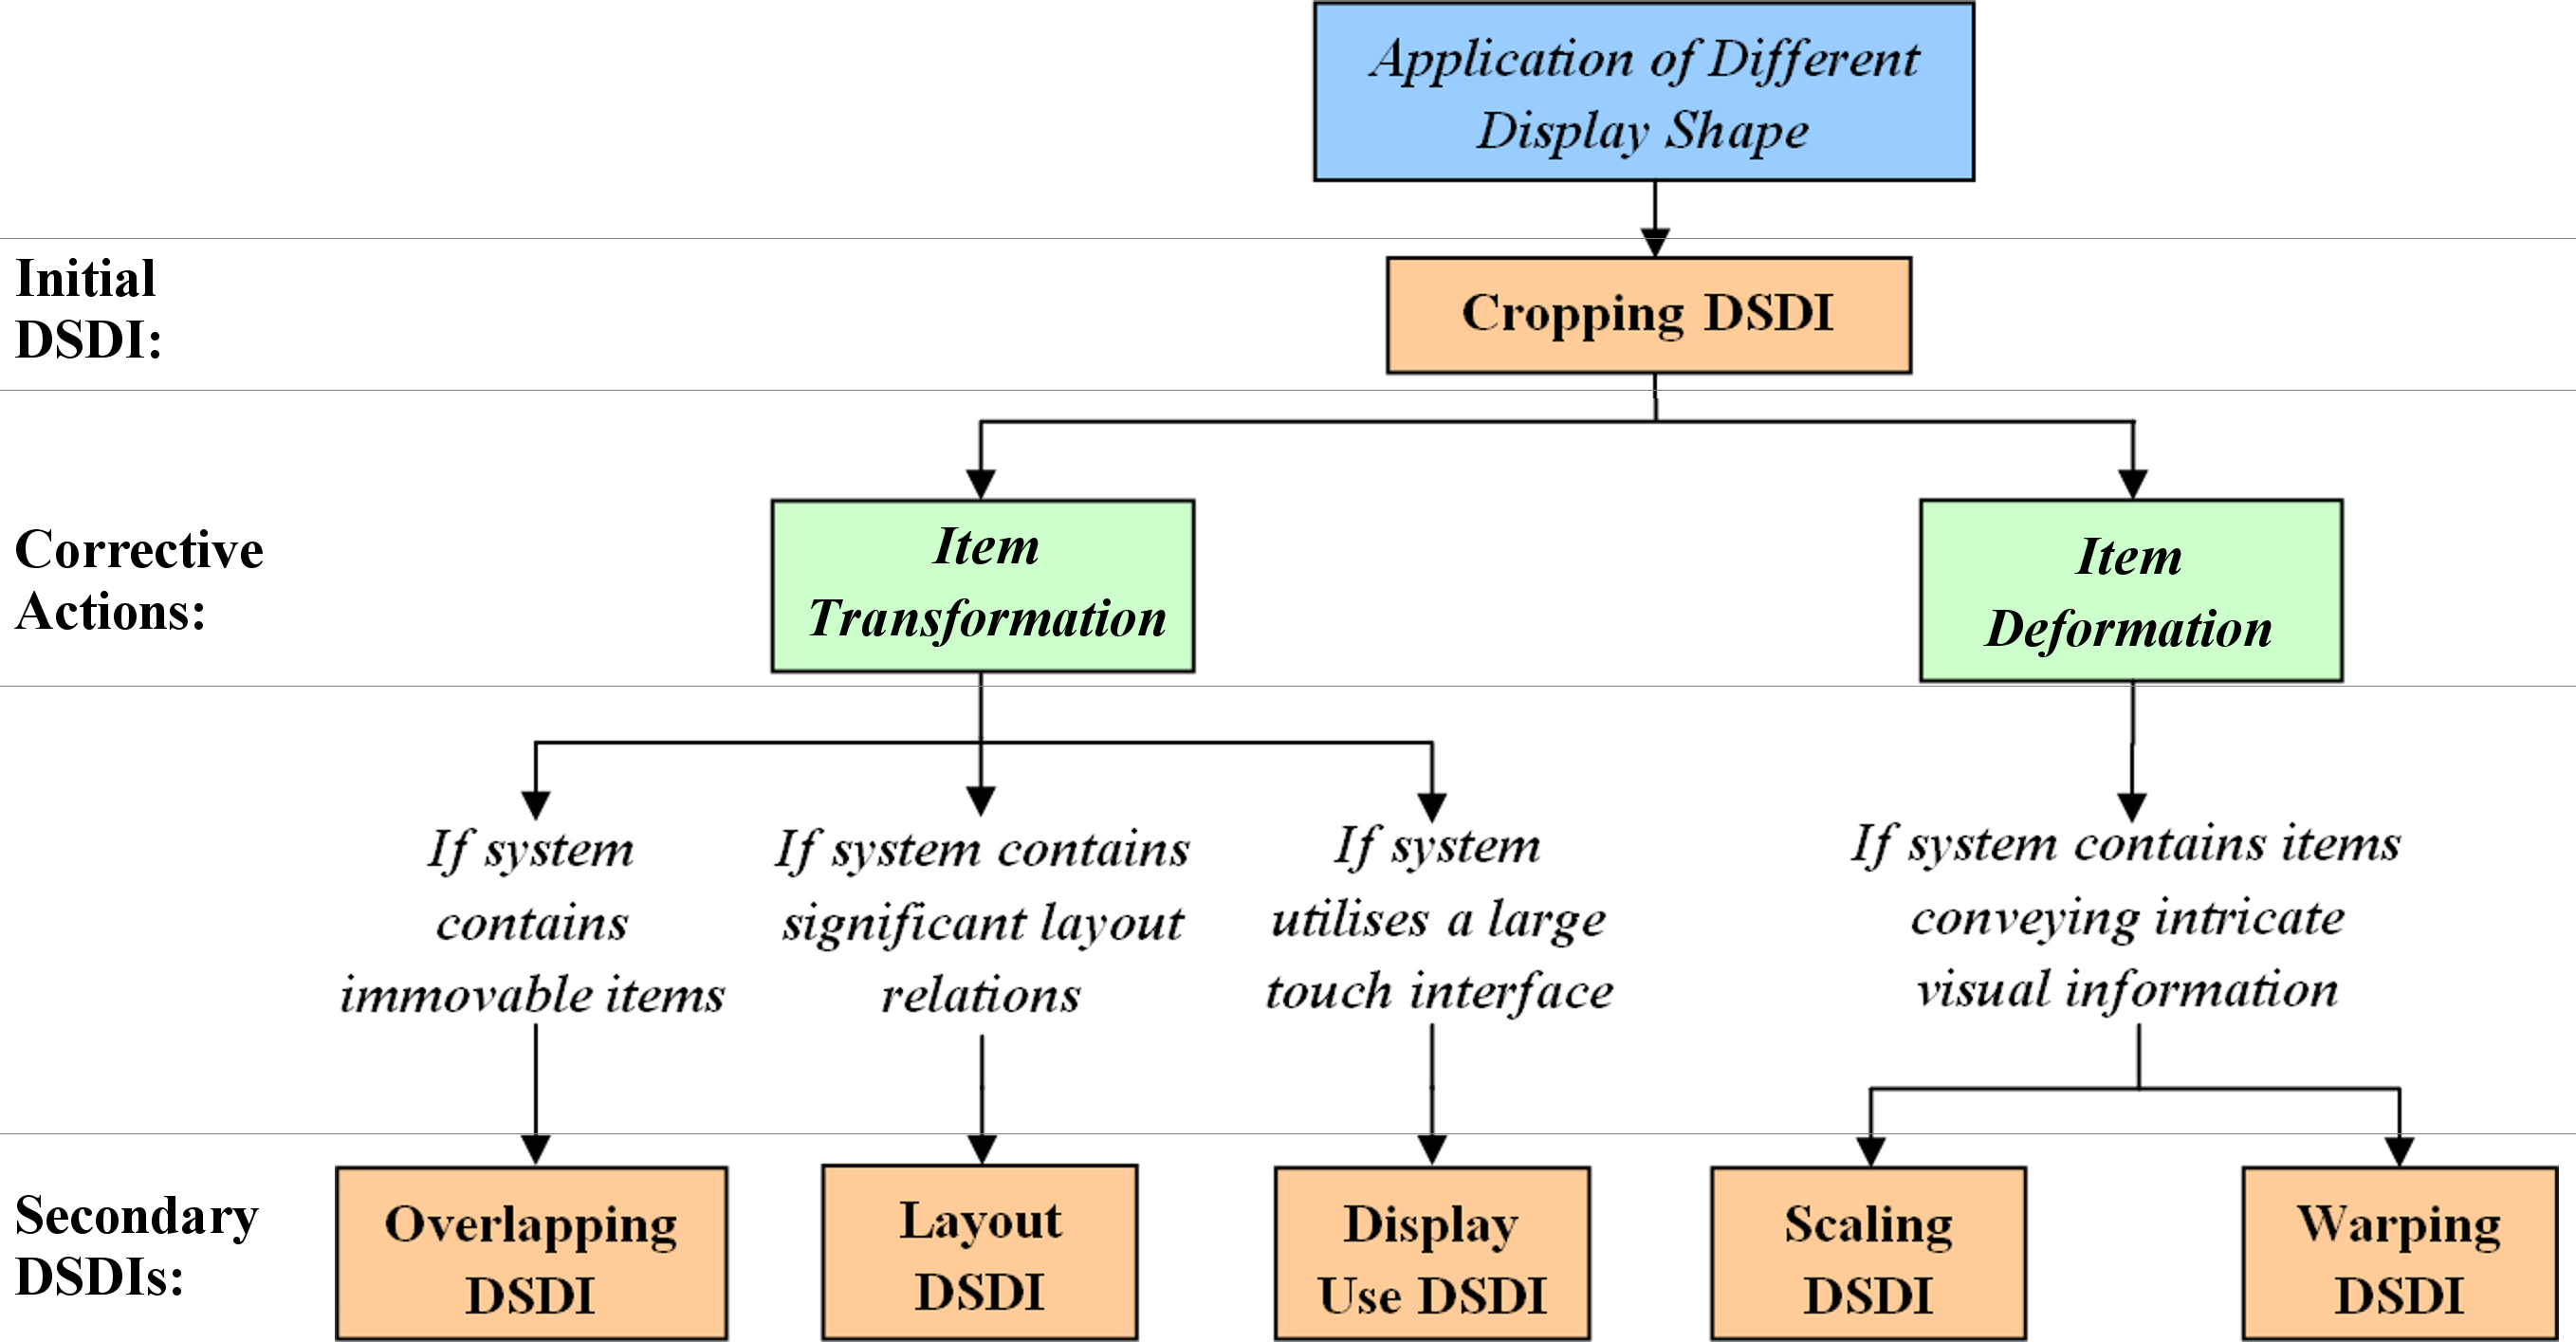
\includegraphics[width=0.95\textwidth]{DSDIFlowChart.png}
   \caption{\csentence{DSDI Flow Chart.}
   A flow chat mapping the causality of Display Shape Dependence Issues (DSDIs).}
   \label{fig:dsdiFlow}
\end{figure}

\begin{figure}[h!]
 \centering
   % 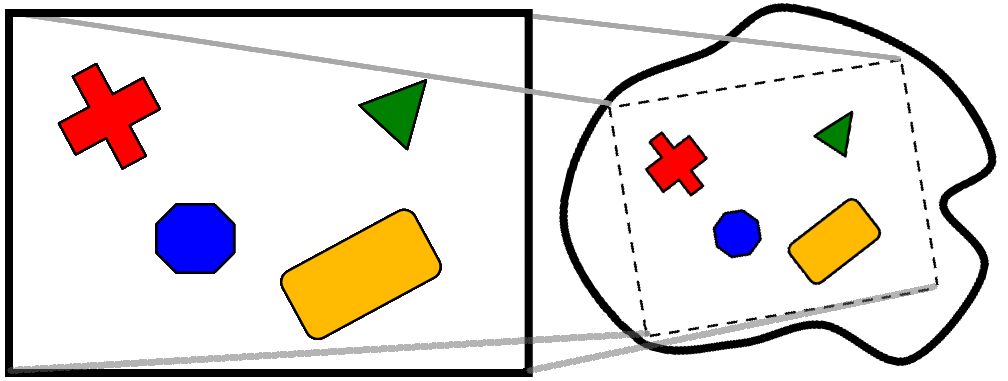
\includegraphics[width=0.45\textwidth]{VirtualProjection.png}
   \caption{\csentence{Virtual Projection.}
   An example of the {\emph{Virtual Projection}} stage.}
   \label{fig:virtualRectangle}
\end{figure}

\begin{figure}[h!] 
 \centering
   % 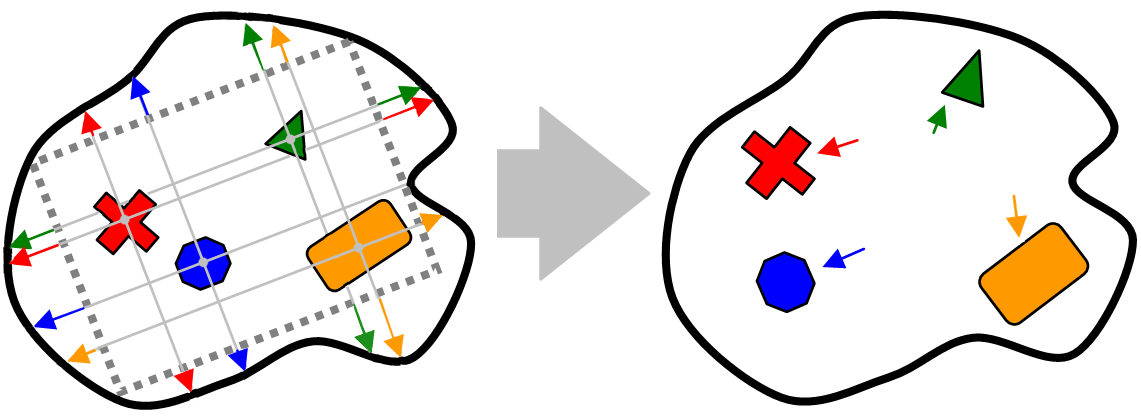
\includegraphics[width=0.45\textwidth]{PositionPulling.png}
   \caption{\csentence{Position Pulling.}
   An example of the {\emph{Position Pulling}} stage.}
   \label{fig:pullLayout}
\end{figure}

\begin{figure}[h!]
 \centering
   % 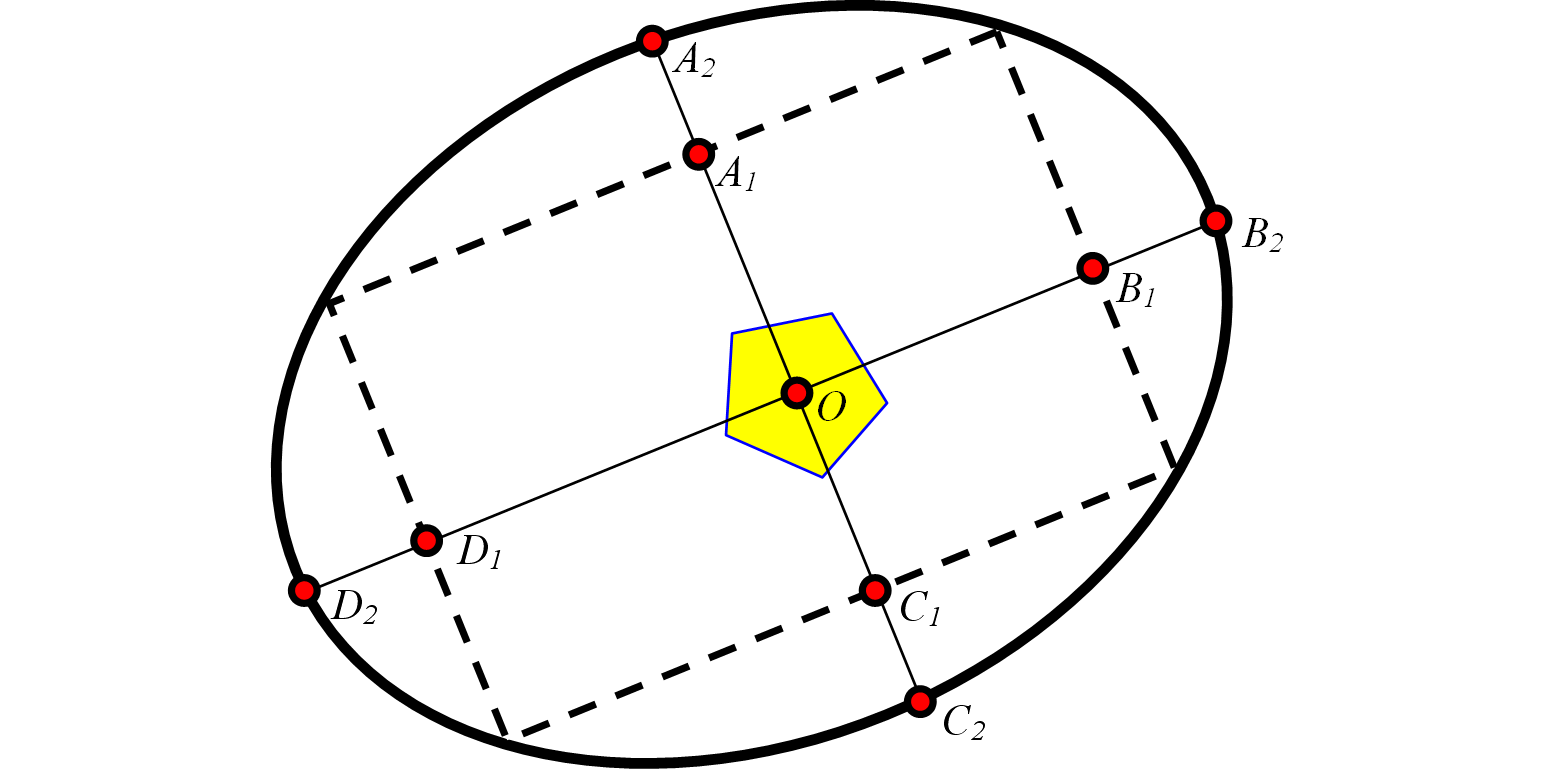
\includegraphics[width=0.45\textwidth]{DetailedPositionPulling.png}
   \caption{\csentence{Detailed Position Pulling.}
   Detailed view of the information used in {\emph{Position Pulling}}.}
   \label{fig:pullLayoutExp}
\end{figure}

\begin{figure}[h!] 
 \centering
  % 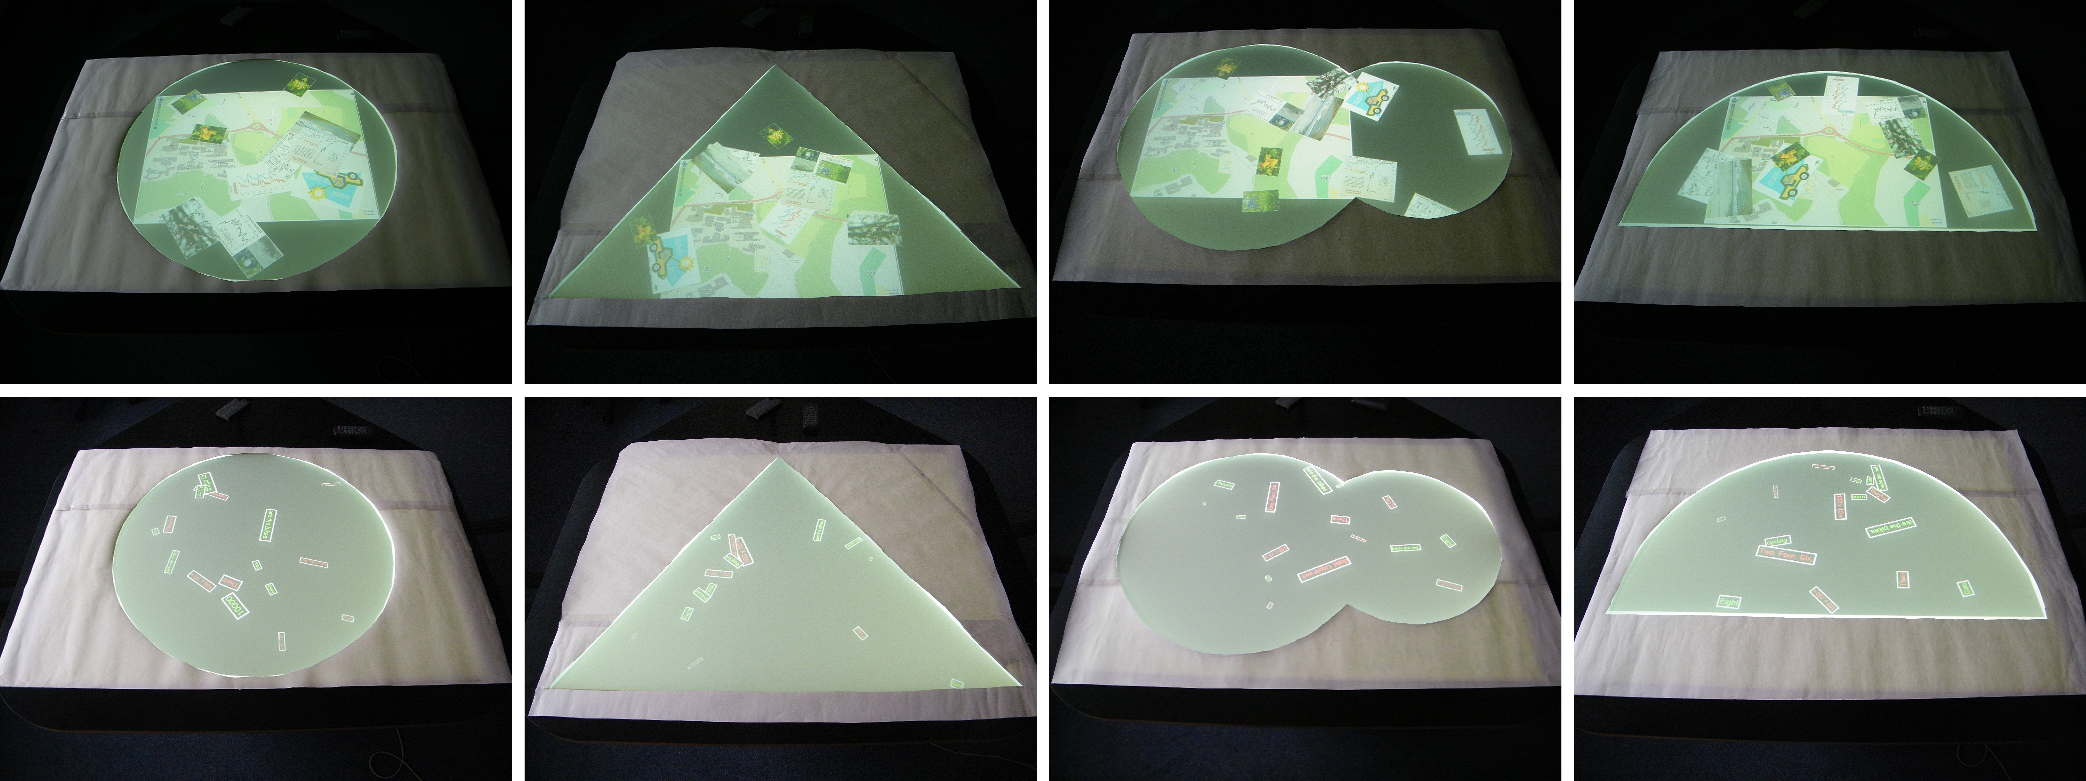
\includegraphics[width=0.95\textwidth]{ApplicationsInUse.png}
  \caption{\csentence{Applications In Use.}
  Several applications in use with different display shapes.}
  \label{fig:trial}
\end{figure}


\begin{figure}[h!] 
 \centering
  % 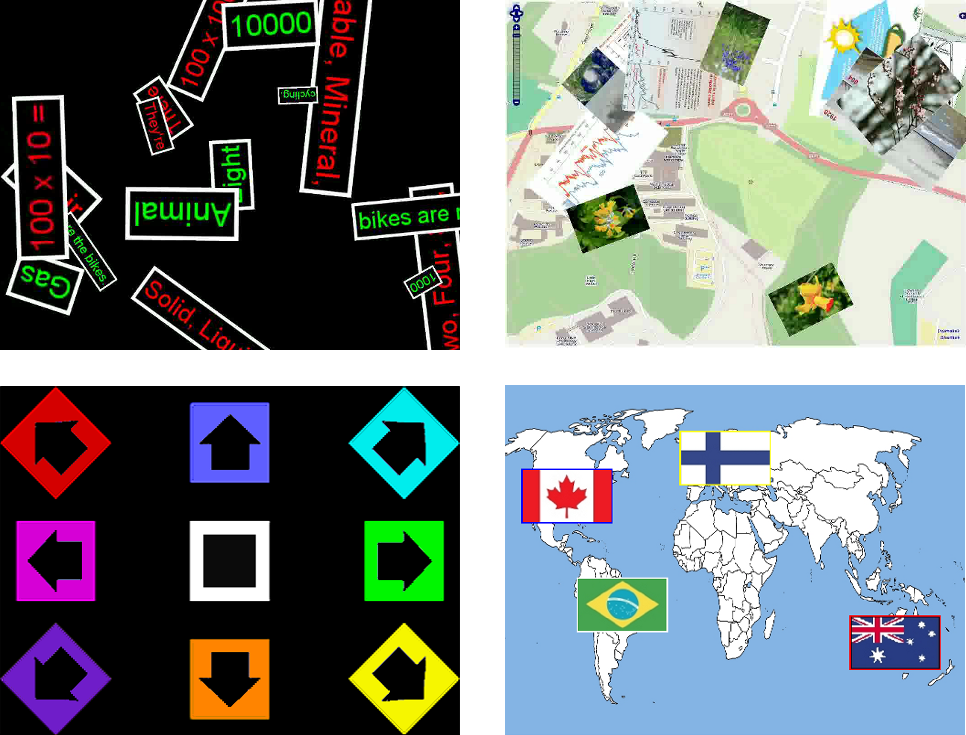
\includegraphics[width=0.95\textwidth]{Applications.png}
  \caption{\csentence{Applications.}
  The applications chosen for observation, from left to right: {\emph{XML Puzzle}}, {\emph{Collage}}, {\emph{Grid}} and {\emph{Simple Map}}.}
  \label{fig:apps}
\end{figure}

\begin{figure}[h!] 
 \centering
  % 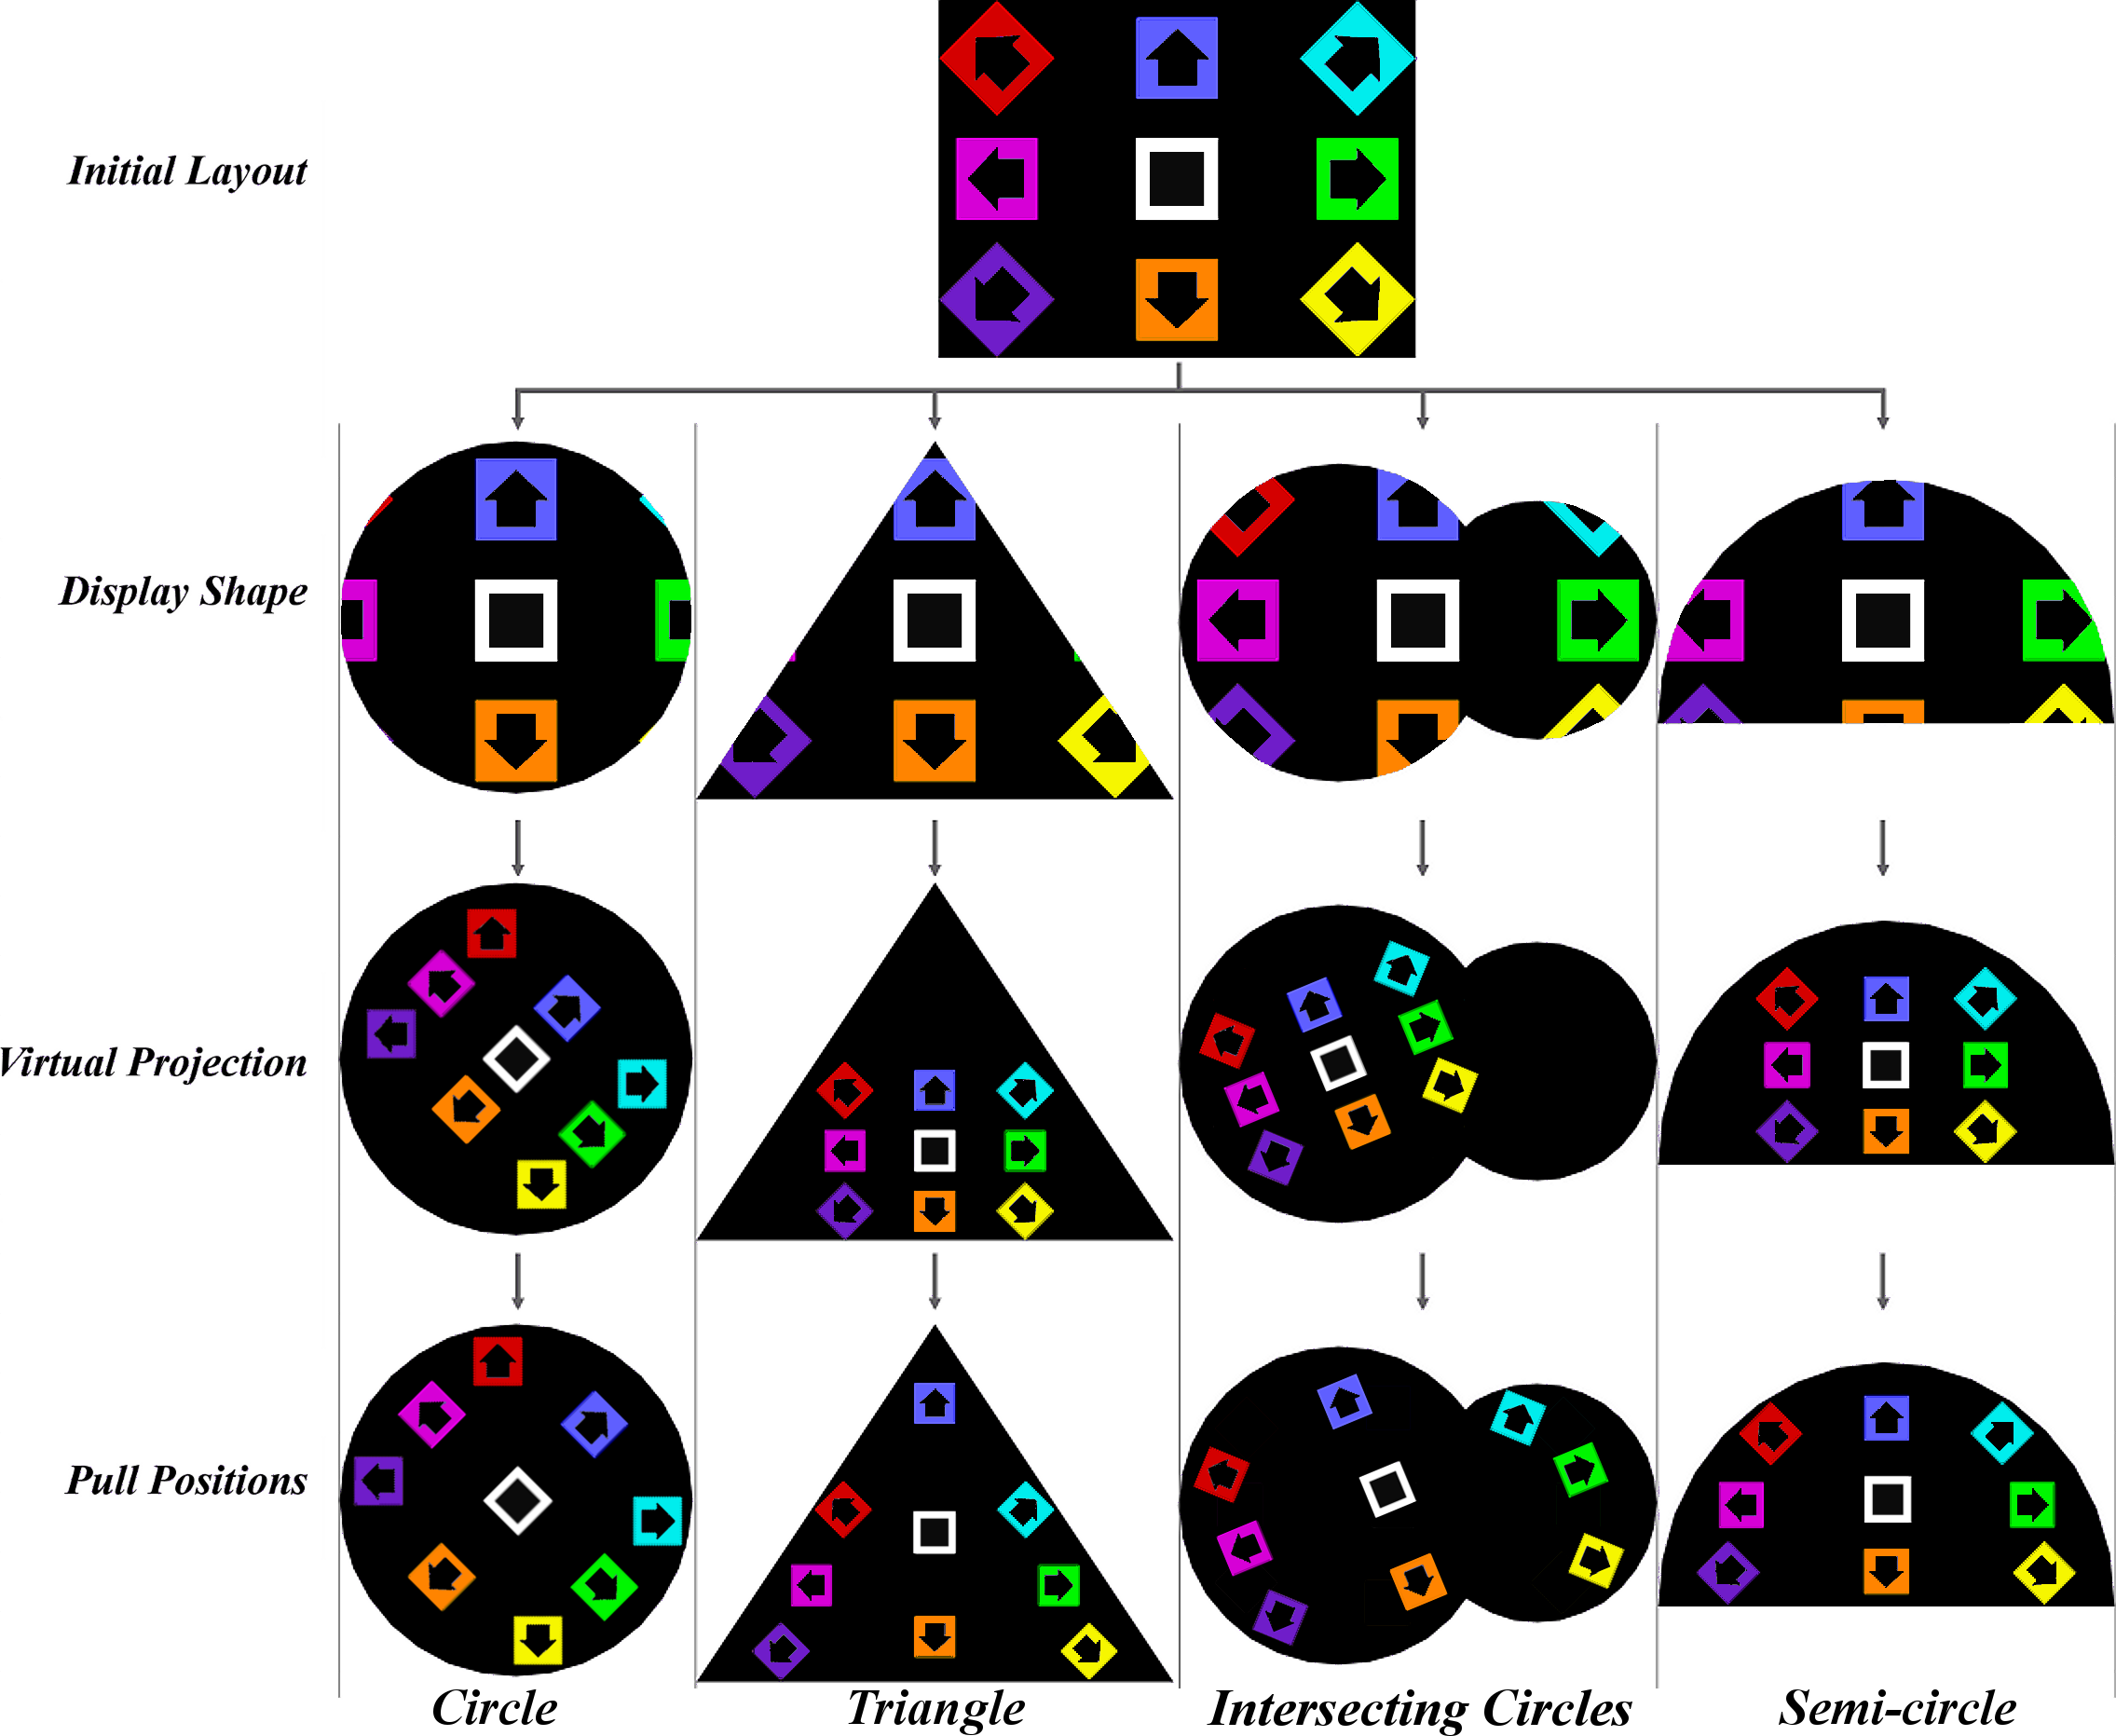
\includegraphics[width=0.95\textwidth]{GridApplication.png}
  \caption{\csentence{Grid Application.}
  Influence of the implemented technique on {\emph{SynergyNet}}'s {\emph{Grid}} application.}
  \label{fig:gridApp}
\end{figure}

\begin{figure}[h!] 
 \centering
  % 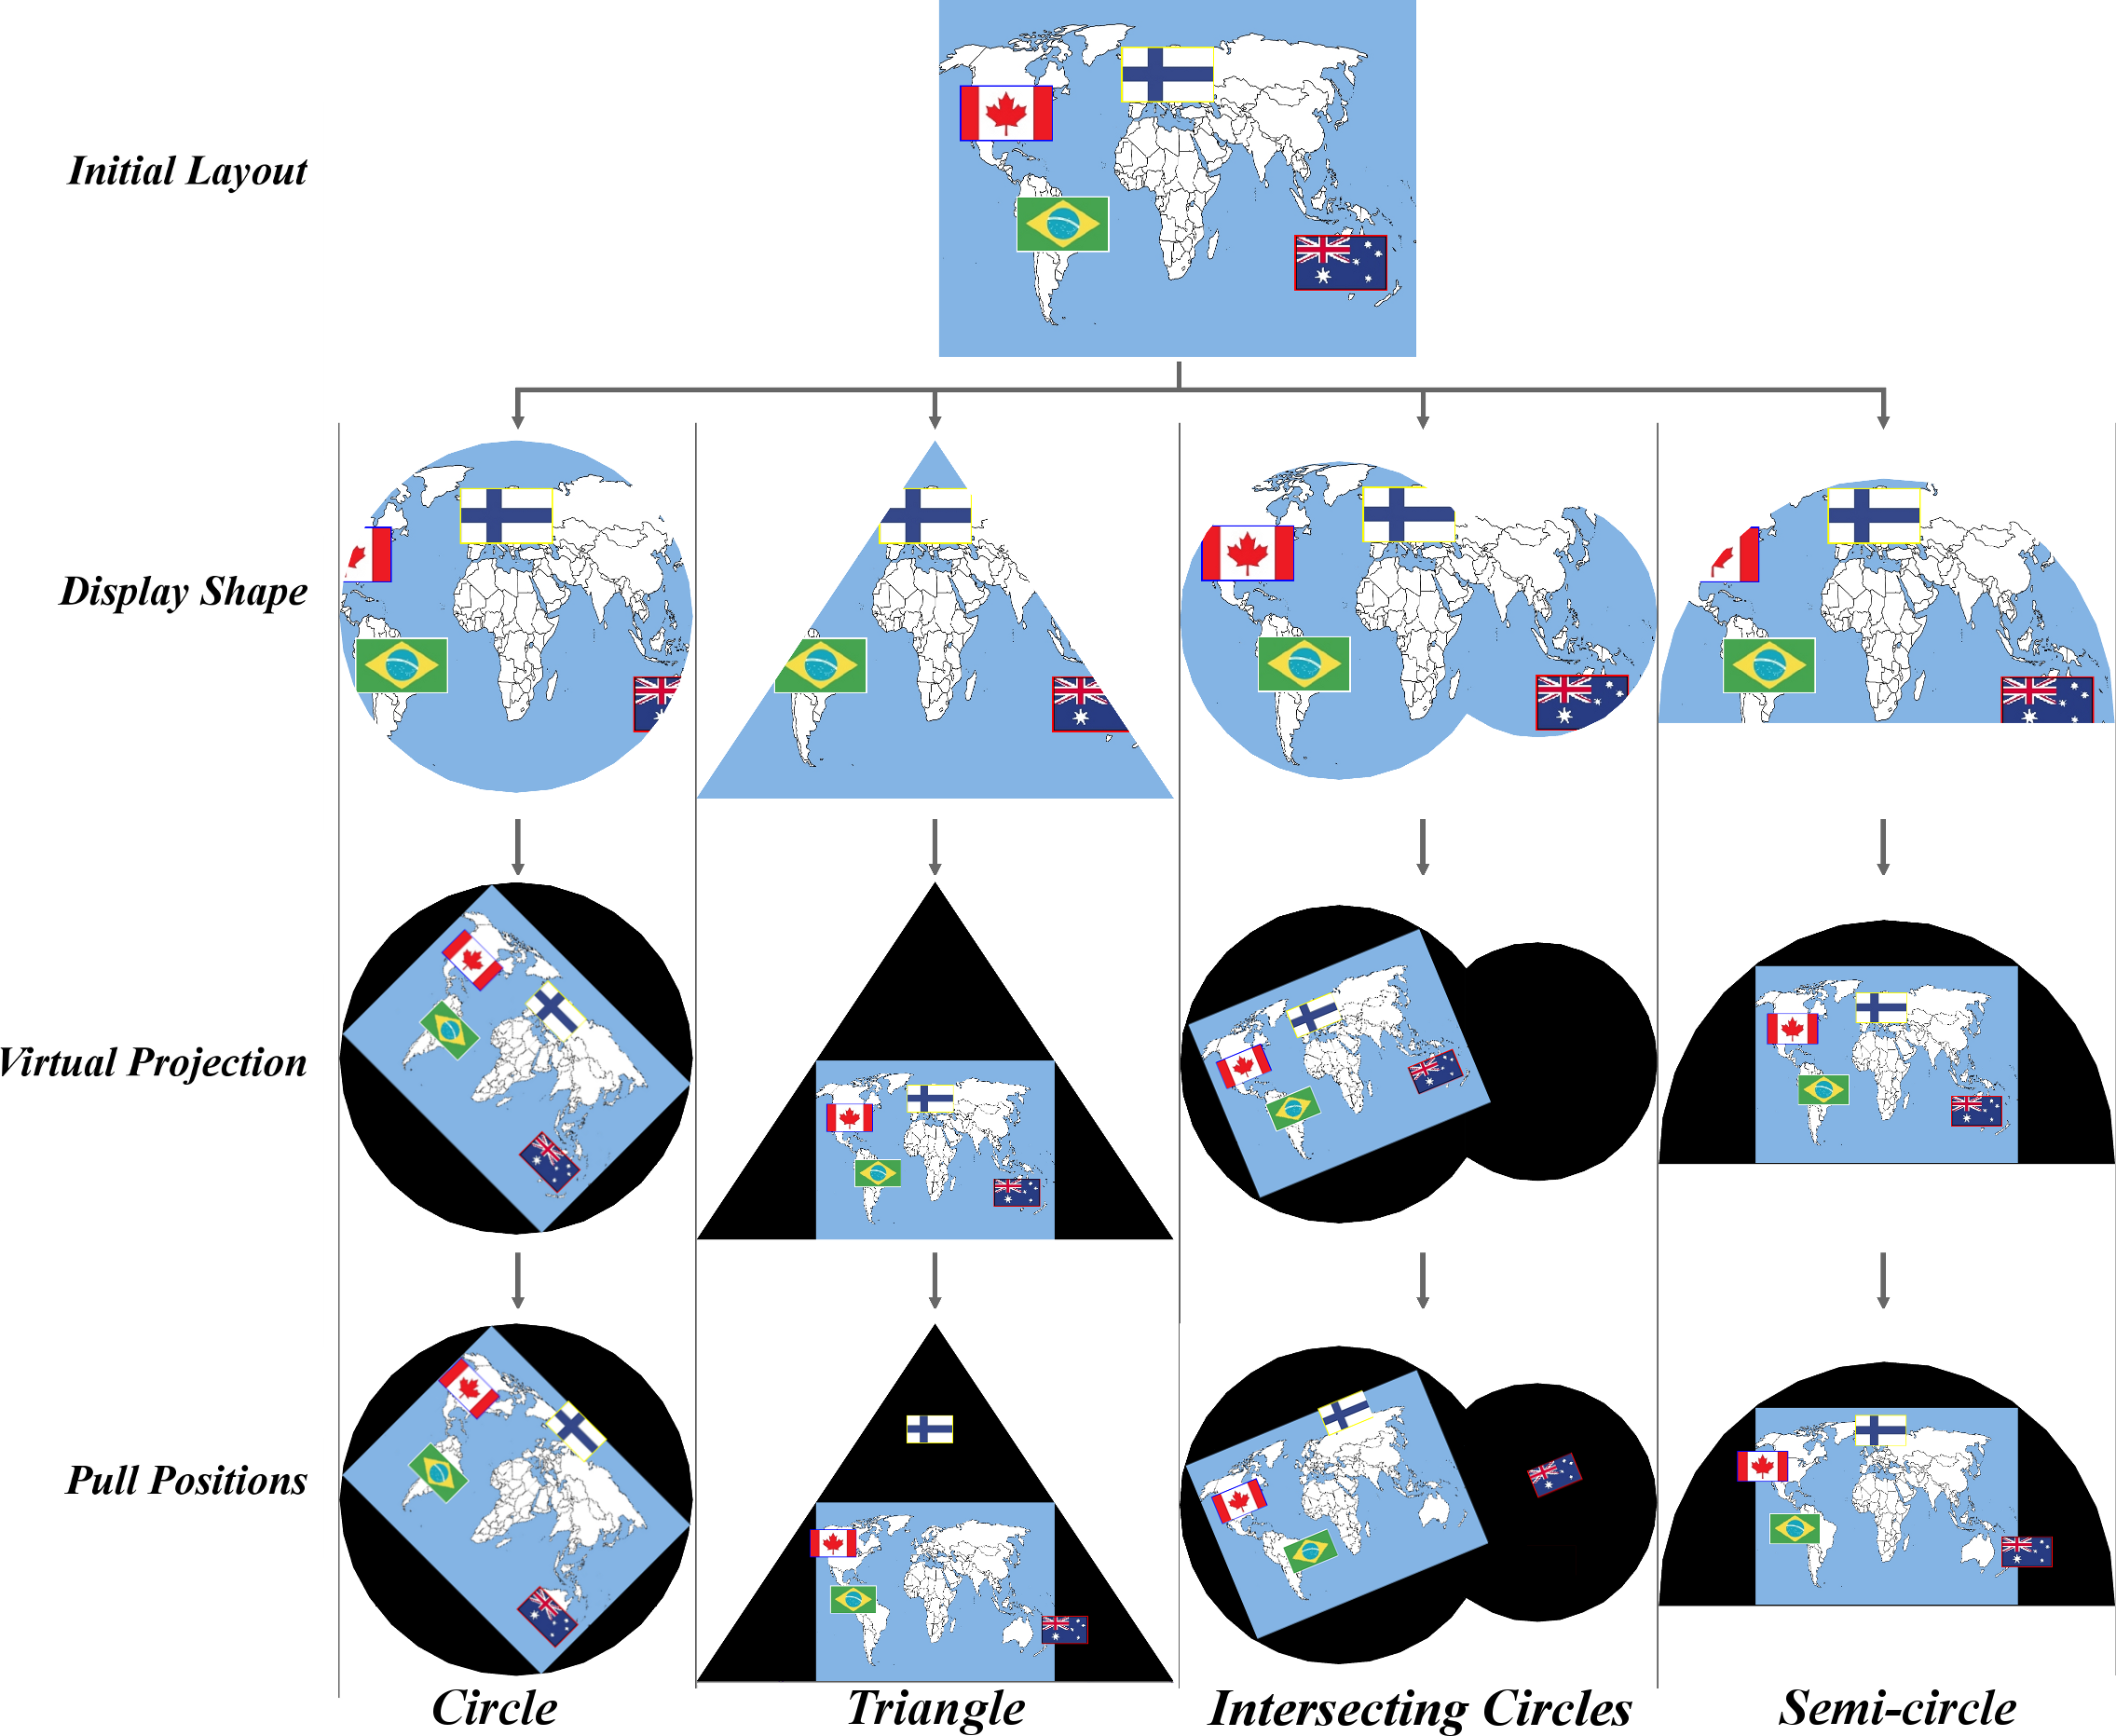
\includegraphics[width=0.95\textwidth]{MapApplication.png}
  \caption{\csentence{Map Application.}
  Influence of the implemented technique on {\emph{SynergyNet}}'s {\emph{Simple Map}} application.}
  \label{fig:mapApp}
\end{figure}

\begin{figure}[h!] 
 \centering
   % 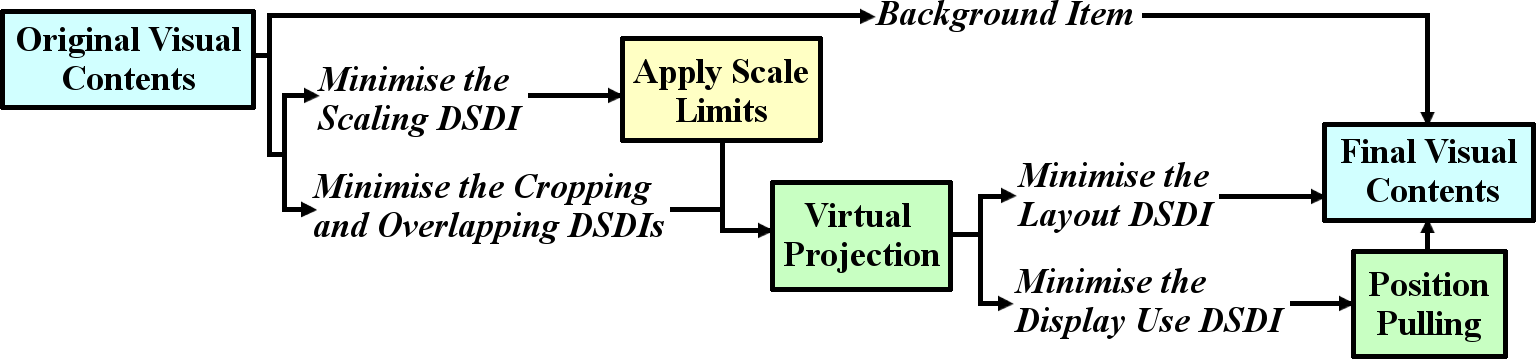
\includegraphics[width=0.95\textwidth]{TechniqueFlowchart.png}
   \caption{\csentence{Technique Flowchart.}
   Flowchart demonstrating navigation of the technique.}
   \label{fig:flowchart}
\end{figure}

\begin{figure}[h!]
 \centering
   % 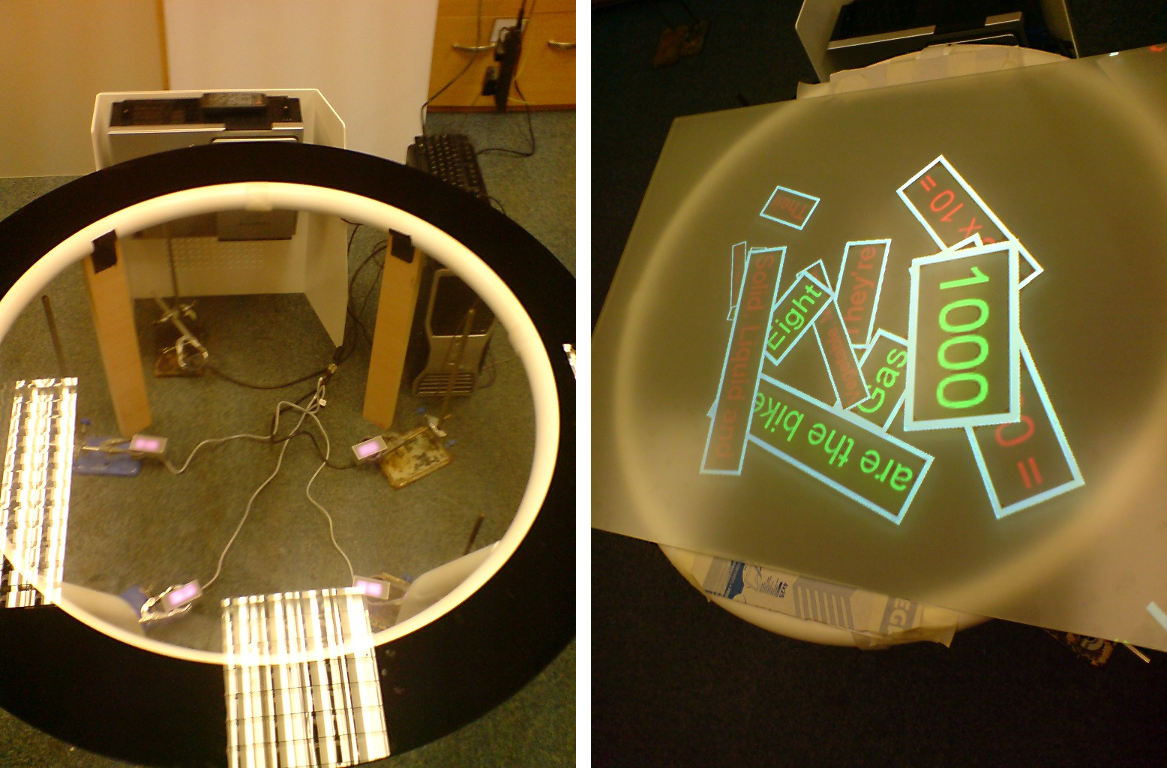
\includegraphics[width=0.45\textwidth]{PrototypeTabletop.png}
   \caption{\csentence{Prototype Tabletop.}
   A prototype of a circular tabletop display.}
   \label{fig:prototypeTabletop}
\end{figure}

%   \begin{figure}[h!]
%   \caption{\csentence{Sample figure title.}
%       A short description of the figure content
%       should go here.}
%       \end{figure}

% \begin{figure}[h!]
%   \caption{\csentence{Sample figure title.}
%       Figure legend text.}
%       \end{figure}

%%%%%%%%%%%%%%%%%%%%%%%%%%%%%%%%%%%
%%                               %%
%% Tables                        %%
%%                               %%
%%%%%%%%%%%%%%%%%%%%%%%%%%%%%%%%%%%

%% Use of \listoftables is discouraged.
%\section*{Tables}

%%%%%%%%%%%%%%%%%%%%%%%%%%%%%%%%%%%
%%                               %%
%% Algorithms                        %%
%%                               %%
%%%%%%%%%%%%%%%%%%%%%%%%%%%%%%%%%%%

%% Use of \listoftables is discouraged.
\pagebreak
\section*{Algorithms}

\begin{algorithm}[h!]
\caption{Calculating the \lq pulling force\rq~vectors.}
\label{algo:pullLayoutOne}
\begin{algorithmic}
\STATE \textbf{getPullVectors}($O,\ A_{1},\ A_{2},\ B_{1},\ B_{2},\ C_{1},\ C_{2},\ D_{1},\ D_{2}$)
\INDSTATE[2]$\overrightarrow{LEFT}\hspace{0.5cm} \leftarrow \hspace{0.25cm}(\overrightarrow{D_{1}D_{2}}\ *\ ( |\overrightarrow{OD_{1}}|\  /\ |\overrightarrow{B_{1}D_{1}}| )$
\INDSTATE[2]$\overrightarrow{RIGHT}\hspace{0.25cm} \leftarrow \hspace{0.25cm}(\overrightarrow{B_{1}B_{2}}\ *\ ( |\overrightarrow{OB_{1}}|\  /\ |\overrightarrow{B_{1}D_{1}}| )$
\INDSTATE[2]$\overrightarrow{UP}\hspace{1cm} \leftarrow \hspace{0.25cm}(\overrightarrow{A_{1}A_{2}}\ *\ ( |\overrightarrow{OC_{1}}|\  /\ |\overrightarrow{A_{1}C_{1}}| )$
\INDSTATE[2]$\overrightarrow{DOWN}\hspace{0.3cm} \leftarrow \hspace{0.25cm}(\overrightarrow{C_{1}C_{2}}\ *\ ( |\overrightarrow{OA_{1}}|\  /\ |\overrightarrow{A_{1}C_{1}}| )$
\STATE \textit{return}\ $\overrightarrow{LEFT},\ \overrightarrow{RIGHT},\ \overrightarrow{UP},\ \overrightarrow{DOWN}$
\end{algorithmic}
\end{algorithm}

\begin{algorithm}[h!]
\caption{Applying the \lq pulling force\rq~vectors.}
\label{algo:pullLayoutTwo}
\begin{algorithmic}
\STATE \textbf{applyPull}($item,\ \theta,\ \overrightarrow{LEFT},\ \overrightarrow{RIGHT},\ \overrightarrow{UP},\ \overrightarrow{DOWN}$)
\INDSTATE[2]$\overrightarrow{PULL} \leftarrow \overrightarrow{LEFT} + \overrightarrow{RIGHT} + \overrightarrow{UP} + \overrightarrow{DOWN}$
\INDSTATE[2]$\overrightarrow{PULL}.rotateBy(\theta)$
\INDSTATE[2]$item.translateBy(\overrightarrow{PULL})$
\STATE \textit{return}
\end{algorithmic}
\end{algorithm}

% \begin{table}[h!]
% \caption{Sample table title. This is where the description of the table should go.}
%       \begin{tabular}{cccc}
%         \hline
%            & B1  &B2   & B3\\ \hline
%         A1 & 0.1 & 0.2 & 0.3\\
%         A2 & ... & ..  & .\\
%         A3 & ..  & .   & .\\ \hline
%       \end{tabular}
% \end{table}

%%%%%%%%%%%%%%%%%%%%%%%%%%%%%%%%%%%
%%                               %%
%% Additional Files              %%
%%                               %%
%%%%%%%%%%%%%%%%%%%%%%%%%%%%%%%%%%%

% \section*{Additional Files}
%   \subsection*{Additional file 1 --- Sample additional file title}
%     Additional file descriptions text (including details of how to
%     view the file, if it is in a non-standard format or the file extension).  This might
%     refer to a multi-page table or a figure.

%   \subsection*{Additional file 2 --- Sample additional file title}
%     Additional file descriptions text.


\end{backmatter}
\end{document}
